\documentclass[letter]{report}
\usepackage{epsfig}
\usepackage{amssymb}

\pagestyle{empty}

\title{ {\LARGE\bf 
        MESQUITE \\ MESh QUality Improvement Toolkit \\ \vspace{.5cm} User's Guide\\
}}

\author{Patrick Knupp, Darryl Melander, Mike Brewer \\
The Sandia National Laboratories \\
Albuquerque NM USA \\
 \\
Lori Freitag-Diachin \\
Livermore National Laboratory \\
Livermore CA USA \\
  \\
Thomas Leurent \\
Argonne National Laboratory \\
Argonne, IL 60490 USA}

\date{Last Updated: 24 June, 2004}

\begin{document}

\maketitle

\tableofcontents

\listoffigures

\listoftables

\chapter{Introduction to Mesquite} \label{sec:intro}

\section{Overview of Mesh Quality}

\hskip 0.25in {\it Mesh quality} refers to geometric properties of a mesh such as 
local volume, smoothness, shape, and orientation that, if not properly 
controlled, 
can adversely affect solution accuracy or computational efficiency of numerical simulations. In this section we give an overview of the role of mesh quality 
in the context of computer simulations of physical phenomena. \newline

Simulation of many phenomena in the physical world involves computing 
numerical 
solutions to partial differential equations (PDE's). Commonly used approaches 
to computing  numerical solutions such as finite volume and finite 
element methods require the use of approximations to the continuum operators 
in the PDE and a mesh or grid to subdivide the physical domain into small 
subregions. Together, the approximations and the mesh define a discretization. 
The difference between the exact solution to the PDE and the numerical solution is known as the discretization error. A {\it convergent} 
discretization means that the discretization error will asymptotically 
approach zero as the characteristic mesh size 'h' 
approaches zero. Decreasing mesh size to reduce discretization error to 
nearly zero is often impractical in realistic simulations due to limited 
computing resources. One way to increase the accuracy of simulations with the 
same computer resources is to {\it adapt} the mesh to the domain and to the 
numerical solution. In adaptive refinement, the local mesh volume (or size) 
is made smaller in locations where the local discretization error is large and 
is made larger in locations where the error is small. In local h-refinement, 
mesh volume is made smaller by locally subdividing the mesh. In 
r-refinement, mesh volume is made smaller by moving mesh nodes closer together.
Geometric adaptation can also be important in improving simulation accuracy. In regions of high domain curvature one adapts the mesh to the domain geometry by creating locally smaller mesh sizes. We see, then, that local mesh size (or volume) is a critical parameter in determining the accuracy of a simulation. \newline

Aside from local mesh size, several other geometric mesh properties can affect 
solution accuracy. These include mesh smoothness, local mesh angles, aspect 
ratio, and orientation. For example, in some discretization methods there will be a 
loss of accuracy if the mesh is not smooth.  In other cases, aspect ratios and 
orientation must be carefully adapted to the solution in order to maintain a 
certain level of accuracy. Simulations using meshes or domains that evolve 
in time (such as in ALE simulations) usually require that initially good 
geometric mesh properties be retained throughout the simulation time period. 
It is thus often important to control other geometric mesh properties in addition to local mesh size within an adaptive simulation. \newline

In addition to solution accuracy, geometric mesh properties can also affect the amount of computer time required to obtain the numerical solution. Simulation codes usually employ iterative solvers to solve systems of equations and thus obtain numerical solutions to PDE's. The rate at which these solvers converge is determined by the spectral radius of a certain matrix. The spectral radius of the matrix is affected by, among other things, geometric properties of the mesh. Poor mesh quality can thus adversely impact solution efficiency. \newline

Adaptive meshing techniques require an initial mesh to begin the adaptation procedure. Poor quality of the initial mesh (relative to the adapted mesh) can be difficult to overcome or, at least, reduce the efficiency of 
the adaptive procedure. For example, if the initial mesh contains locally inverted elements, these can often be fixed before the adaptive procedure begins. As another example, if it is known \`{a} priori that small angles will be needed on the boundary of the domain to obtain reasonable simulation accuracy, one should try to first create the small angles in the initial mesh to improve the efficiency of the subsequent adaptive meshing procedure. \newline


Many simulations, particularly those in industry, are performed in a 
non-adaptive setting. That is to say, an initial mesh is generated and
used throughout the calculation. The mesh is not changed as the solution
is computed. Mesh quality remains important for such calculations. First, 
for complicated geometric domains it is often difficult to obtain good 
initial mesh quality. This is particularly true for non-simplicial meshes 
but can be true for simplicial meshes as well. A common requirement is that the mesh be smooth. Many simulation codes will not run to completion if the initial mesh contains a local volume which is negative. These must be eliminated before a simulation can begin. Analysts performing 
non-adaptive calculations often have considerable experience in using a variety
of meshes on their problem and have a good \`{a} priori idea of what constitutes
good mesh quality for a given problem. They thus desire to control the usual
geometric mesh properties of the non-adapted mesh carefully. 



\section{How Mesh Quality Is Improved}
Mesh quality can and should be considered during many stages of 
the mesh generation process from de-featuring CAD models to  
creation and adaptation of the mesh. Thus, for example, certain
non-essential features of a CAD model, if eliminated, would go a 
long way to improving the quality of the mesh, depending upon
the meshing scheme. Other critical meshing parameters which can 
affect mesh quality include geometric domain partitions, interval size
and count, interaction of meshes within large assemblies of parts, 
biasing requirements, corner picking, etc. Choices made during the 
mesh generation phase of an analysis may have a large impact on 
initial mesh quality.  Mesh quality can thus be improved by changing the 
way in which the domain is meshed. \newline

Once the meshing stage is completed, one can improve mesh quality
by techniques such as vertex movement and local topology modification.
In vertex movement schemes, one seeks to reposition existing mesh vertices to 
achieve better quality. If vertex movement is undertaken within an adaptive 
setting, it is commonly referred to as r-refinement. 
Classic examples of vertex movement methods 
include Laplace smoothing \cite{F88} and Winslow smoothing \cite{Winslow}. 
It is helpful, in vertex movement schemes, to first be 
able to measure mesh quality so that one can explain in what sense one 
has improved it. Given a {\it metric} to measure mesh quality, 
one can formulate a numerical 
optimization problem which guides vertex movement to find the optimal 
mesh and thus improve its quality.  Numerical 
optimization methods recently
developed for unstructured meshes include \cite{Opt-MS,Kn00,FrKn01,
FeasNewt,bjoe:swap,bjoe:chain-swap,es92}. We refer the reader to ref xxx
which is a survey of mesh quality improvement methods which have appeared 
in the literature. \newline

A large number of mesh quality metrics have been devised to measure 
mesh quality. Many of these metrics are independent of any solution 
properties and are thus not useful in adaptive meshing. However, there
are a number of weighted quality metrics which can be tied to the 
numerical solution via error indicators or other information for adaptive 
meshing. Examples of weighted metrics which have or could be used in 
adaptive calculations include those of Brackbill (ref), Knupp (ref), etc. \newline

Another way to improve mesh quality is to use local topological modification methods in which mesh vertices or elements are locally created and/or destroyed. These methods are very successful when applied to simplicial meshes, often within an adaptive context.  Local topology modification is less effective on non-simplicial meshes. \newline

Mesh quality improvement remains an important on-going research area. 
There remain, for example, open questions with regard to metrics which 
can be used in adaptive settings, theoretical questions on problem 
formulation, and how to obtain improved meshes quickly. \newline

Although mesh quality improvement algorithms have been widely implemented 
in both meshing and applications codes, it has always been difficult to 
improve the quality of a mesh created in one software package using an 
improvement algorithm which has been implemented in another.  This difficulty
and others have inspired the creation of the Mesquite software library. 
This library is described in the next section. \newline


\section{Mesquite Goals}
Mesquite (Mesh Quality Improvement Toolkit) is designed to provide a
stand-alone, portable, comprehensive suite of mesh quality improvement
algorithms.  The design flexible so that they can be applied to many
different mesh element types and orders and referenced to both
isotropic and anisotropic ideal elements.  Mesquite provides a robust
and effective mesh improvement toolkit that allows both meshing
researchers application scientists to benefit from the latest
developments in mesh quality control and improvement. \newline

Mesquite design goals are derived from a mathematical framework and
are focused on providing a versatile, comprehensive, inter-operable,
robust, and efficient library of mesh quality improvement algorithms
that can be used by the non-expert and extended and customized by
experts.  In this section we highlight the current status of Mesquite
in several of our design goal areas. \newline


{\bf Versatile.}  Mesquite works on structured, unstructured, and
hybrid meshes in both two and three dimensions. The design permits
improvements to meshes composed of triangular, tetrahedral,
quadrilateral, and hexahedral elements. Prismatic, pyramidal, and
polyhedral elements can be easily added.  It currently incorporates
only methods for node movement; plans for topology modification and
hybrid improvement strategies lie in the future.  Node movement
strategies include both local patch-based iteration schemes for one or
a few free vertices and global objective functions which improve all
vertices simultaneously. Mesquite will be applicable to both adaptive
and nonadaptive meshing and to both low- and high-order discretization
schemes, but currently works with non-adaptive meshes containing
linear elements. \newline

{\bf Comprehensive.}  Mesquite will address a large variety of mesh
quality improvement goals including mesh volume control (sizing,
invertibility), mesh angles, aspect ratios, and orientation. Specific
goals include mesh untangling, mesh smoothing, shape improvement,
anisotropic smoothing, mesh rezoning for ALE, mesh alignment, and
deforming mesh algorithms. These goals can be pursued in both adaptive
and non-adaptive settings. The software is customizable, enabling
users to insert their own quality metrics, objective functions, and
algorithms and also provides mechanisms for creating combined
approaches that use one or more improvement algorithms. \newline

%{\bf Effective.}  Mesquite uses state-of-the-art algorithms and
%metrics to guarantee improvement in mesh quality.  Because the
%definition of mesh quality is application specific, we provide quality
%metrics that allow the user to untangle meshes, improve mesh
%smoothness, element size, and shape. In the future these metrics will
%be referenced to permit non-isotropic smoothing and adaptivity. \newline

{\bf Inter-operable.}  To ensure that Mesquite is inter-operable with a
large number of mesh generation packages, we use the common
interfaces for mesh query currently under development by the TSTT
center.  These interfaces provide uniform access to mesh geometry and
topology and will be implemented by all TSTT center software including
several DOE-supported mesh generation packages.  We are working with
the TSTT interface design team to ensure that Mesquite has efficient
access to mesh and geometry information through strategies such as
information caching and agglomeration.  We are also participating in
the design of interfaces needed to support topological changes
generated by mesh swapping and flipping algorithms and to constrain
vertices to the surface of a geometrical model. \newline

{\bf Efficient.}  The outer layers of Mesquite use 
object-oriented design in C++ while the inner kernels use
optimizable coding constructs such as arrays and inlined
functions.  To ensure efficient use of computationally intensive
optimization algorithms, we employ inexpensive smoothers, such as
Laplacian smoothing, as ``preconditioners'' for the more expensive
optimization techniques.  In addition, mesh culling algorithms can be
used to smooth only those areas of the mesh that require improvement.
Considerable attention has been devoted to understanding and
implementing a variety of termination criteria that can be used to
control the computational cost of the optimization algorithms. \newline

{\bf Robust.} Sound software engineering principles and robust numerical 
algorithms are employed in Mesquite. 
%Code interrupts due to null pointers and zero-divides will be handled gracefully.  
A comprehensive suite of test problems and a unit testing framework have
been developed to verify the correct execution of the code. \newline

Mesquite is not intended to be a mesh generation tool. It can serve as 
a post-processor to a mesh generation procedure, a mesh pre-processor to a 
non-adaptive simulation code, or as an algorithm for in-core adaptive mesh 
quality improvement. As a software library, Mesquite is intended to be
linked to either a meshing code or to a simulation code. \newline

\section{Mesquite Concepts} \label{sec:concepts}

Mesquite software design is based on a mathematical 
framework that improves mesh quality by solving an optimization 
problem to guide the movement of mesh vertices \cite{formal}. 
The user inputs a mesh or 
submesh consisting of vertices, elements, and the relationships between them. 
The quality of each vertex or 
element in the mesh is described by a local quality metric that is a function 
of a subset of the mesh vertices. The global quality of the mesh is formed by 
taking the global norm or the average of the local mesh qualities. The global 
quality is thus a function of the positions of all the mesh vertices. If this 
function can be used in a well-posed minimization problem (e.g., it is 
bounded below and has one or more local minimums), mesh vertices are moved 
by Mesquite toward the vertex positions of the optimal mesh, thus improving 
the quality according to the criterion defined by the local quality metric. 
By changing the local quality metric one can achieve a variety of mesh quality improvement goals such as mesh untangling, shape improvement, and size adaptation. \newline

Users of Mesquite should have in mind a goal or set of goals which define 
the quality of the mesh which is to be improved. The goal determines which
quality metric or metrics one will use in the optimization problem. Other 
user inputs will include an objective function template which describes 
the norm or average they wish to use in defining the global mesh quality. 
For example, an L-infinity norm will tend to improve the worst-case local 
quality while an L-2 norm will improve the RMS quality of the global mesh. 
Once the global quality (objective function) is defined, the user can 
select a numerical optimization scheme (solver) within Mesquite such as a 
steepest descent, conjugate gradient, or feasible Newton method. A variety of 
termination criteria can be selected singly or in combination to tell the 
solver when to halt. These are useful in controlling the trade-off between
the accuracy of the minimization procedure vs. how much CPU is consumed. 
There is also an important flag that determines whether the optimization 
problem will be solved via a succession of optimizations on local patches 
followed by a complete pass over the global mesh or if it will be solved using 
a global patch in which all mesh vertices are moved simultaneously. Advantages
and disadvantages of each of these approaches is currently under study.\newline

Sometimes hybrid mesh optimization schemes are useful, for example, in 
first untangling a mesh and then improving the shape of its elements. For 
sequences of optimization problems Mesquite uses the concept of an 
instruction queue.  The queue determines the order in which the optimization
problems are solved, using the output from the previous optimization step 
as the input to the next optimization step. The queue defines a master 
quality improver that defines the ultimate mesh quality improvement goal.
The queue can also be used to include steps to assess mesh quality say 
before and after each optimization step within the queue.  The quality 
assessor measures various aspects of quality in the mesh and may include 
other quality metrics besides the one used to define the optimization problem.
\newline

Optimization problems can be solved directly by minimizing the objective 
function or indirectly by positioning mesh vertices at a stationary point
of the global objective function. Stationary points are defined by setting 
the gradient of the objective function to zero. The indirect method is akin 
to iteratively solving a system of linear (or nonlinear) equations. 
Currently, such systems are solved in Mesquite and other mesh quality 
software by using the local patch method that is akin 
to a Gauss-Seidel iteration. The prime example of this in Mesquite is 
Laplace smoothing. In the 
future we may include methods for solving global systems of equations 
in Mesquite to obtain solutions more quickly. 
In the past, some mesh smoothing algorithms have been formulated as a 
local iterative method that cannot be derived  
by setting the gradient of an objective function to zero. Such methods are
frowned upon in Mesquite since one cannot state what mesh quality metric is
improved.  However, if such methods are included in future version sof Mesquite, they will be done in a manner similar to the local Laplace smoothing 
algorithm in Mesquite. \newline

\noindent The following notation is used in the rest of this manual
\begin{itemize}
\item The mesh is assumed to consist of $N$ elements and $M$ free vertices.  
Let $n=1,2,\ldots,N$.
\item Let $q$ be a scalar which defines an element-based {\it quality} metric. 
The quality of the $n^{th}$ element in the mesh is given by the scalar 
$q_n$. Element quality is a function of the coordinates ${\bf x}_n$ 
of the vertices belonging to the element, i.e., $q_n = q({\bf x}_n)$
\item Let $Q \in R^N$ be the vector $[q_1,q_2,\ldots,q_n]$ of element 
qualities over the mesh. Let $f$ be a function from $R^N$ to $R$. When  
$f$ is applied to $Q$, we call $f(Q)$ an {\it objective function template}.
\item Because each of the element qualities depends on the coordinates of
the vertices which it contains, the vector $Q$ is a function of the coordinates
of all of the free vertices ${\bf x} \in R^{3M}$ in the mesh, i.e., $Q=Q({\bf x})$. Finally, form $F({\bf x})= f \circ Q({\bf x}) = f(Q({\bf x}))$ as a 
function from $R^{3M}$ to $R$.  The function $F$ is the mesh quality 
{\it objective function}. 
\item $\nabla F \in R^{3M}$ is the {\it gradient} of the objective function 
with respect to the coordinates of the free vertices. Let ${\cal H} F= \nabla (\nabla F)$ be the {\it Hessian} of the objective function.  The Hessian is a 
$3M \times 3M$ matrix. 
\end{itemize}

\begin{figure}[htb]
\begin{center}
\begin{tabular}{c}
\psfig{figure=./msq-paradigm.eps,width=4.7in}
\end{tabular}
\end{center}
\caption{\em The Mesquite Paradigm \label{Paradigm} }
\end{figure}

\section{How to use this User's Manual}
This user's manual 
\begin{itemize}
\item provides an introduction to mesh quality and basic Mesquite concepts (chapter \ref{sec:intro}), 
\item instructs novice users on how to download and compile
Mesquite. A tutorial is given of Mesquite simplified user's interface and Mesquite's detailed API (chapter \ref{sec:basics}).
\item describes how to load a mesh in Mesquite via files (section \ref{sec:meshFiles}), 
\item provides instructions on using the extensive TSTT interface or a Mesquite mesh specific mesh
      interface to load a mesh dynamicallu in Mesquite (sections \ref{sec:msq_mesh}, \ref{sec:TSTT}).
\item describes Mesquite interactions with domain geometry (Section 3.4),
\item Exposes in details the concepts and the mechanisms of the advanced API (chapter \ref{sec:API}), and 
\item instructs the user on how to add their own instances of quality 
metrics, objective functions, and solvers (chapter \ref{sec:extensions})
\end{itemize}

Consult the doxygen documentation for the API reference as well as details on the software. There
are two sets of doxygen documentations available:
\begin{itemize}
\item The developer doxygen doc is located in mesquite/doc/developer/. From that directory, you
      must run 'doxygen Mesquite.dox'.
\item The user doxygen doc (API doc) is located in mesquite/doc/user/doxygen. From that directory, you
      must run 'doxygen Mesquite-user.dox'.
\end{itemize}
The doxygen command will generate two directories: an html directory containing the file
index.html that you can open with your web browser, and a latex directory containing a Makefile that
will generate a dvi file. 
\newline


\chapter{Basic Mesquite Usage} \label{sec:basics}

\section{Downloading Mesquite}

\subsection{System Requirements}
TODO:  List the supported platforms (Lin, SGI, Sun, etc.?), the required
software (makedepend, gmake, Babel, etc.?), and any related information.
\subsection{Acquiring the Necessary Code/Libraries}
TODO:  How and where Mesquite, AOMD, CppUnit, (MDB), etc. can be
acquired... with appropriate acknowledgments.

\section{Compiling and Linking Mesquite}
\label{sec:compiling}
\begin{verbatim}
TODO:  Software dependencies, compiling AOMD, TSTT interfaces
(need the .h file), other (gmake, makedepend)?  
Makefiles (examples that link Mesquite to an 
application code). Compiler flags and options (debugging, profiling). 
Platforms supported. Optional functionalities (debugging, profiling, 
error handling).
\end{verbatim}

Having acquired the Mesquite source code, the user can perform the
following steps which outline the process for compiling the code and
creating the library, `libmesquite.a'. Here is the fastest way to compile Mesquite:
\begin{enumerate}
\item While in the top level Mesquite directory (typically, .../mesquite/), type
`./configure'.  This will create the file Makefile.customize with a default configuration
for your platform.
\item Type gmake, this will compile the library lib/libmesquite.a
\item To compile, one of the test, stay in the main directory (mesquite/) and type 
for example 'gmake testSuite/test\_1/main'. You can also use 'gmake all\_tests' .
\end{enumerate}
If the above worked, you are done. Mesquite compiled successfully. 

If the above method did not work for your system, you will have to modify the file
Makefile.customize that contains the platform specific tools and settings to be used 
while compiling Mesquite. In the remainder of this section, we
will  list some of the specific variables which
may need to be modified before Mesquite will compile correctly.
This can be done in two ways: you can use the configure
script options (you can access these options and
others by typing './configure --help'), or you can edit
Makefile.customize directly.

\subsection{Basic Configure Options.}  \label{config_options}

Those options can be given to the configure script through the command line, for example the C headers
option would be given by typing \texttt{./configure --with-c-headers=yes} in the \texttt{mesquite/} directory.

\begin{description}
\item \texttt{--with-c-headers=yes} Uses the deprecated C style for headers:
  will use headers like \texttt{<inostream.h>} and \texttt{<math.h>}
  instead of the new C++ style \texttt{<iostream>} and \texttt{<cmath>}. This might make older
  compilers find those headers. With newer compilers, you will get a warning for using deprecated headers.
\item \texttt{--with-makedepend=EXECUTABLE}  Location of alternative makedepend program:
Give the full path:  --with-makedepend='/usr/local/bin/makedepend'
\item \texttt{--with-archiver=EXECUTABLE} Location of alternative archiver (default is 'ar ru'):
Give the full path: --with-archiver='/usr/local/bin/ar' . If options are needed, we advise to
create a shell script pointed to by that option. The shell script would contain only one line: the
archiver and its options. 
\item \texttt{--with-cc=EXECUTABLE}  Location of alternative C compiler:
Give the full path: --with-cc='/usr/local/gcc/bin/gcc'
\item \texttt{--with-cPP=EXECUTABLE}  Location of alternative c++ compiler:
Give the full path:  --with-cPP='/usr/local/gcc/bin/g++'
\item \texttt{--with-dox=EXECUTABLE}  Location of doxygen:
Give the full path: --with-dox='/usr/local/bin/doxygen'
\end{description}

For all configure options, type
\begin{verbatim}
./configure --help
\end{verbatim}
Also, configure options for the TSTT linking are described in section \ref{sec:TSTT}.



\subsection{Basic Makefile Variables.}  \label{mes_vars_and_defs}

The following is a list of variables used in Mesquite's Makefile
structure to allow for customization of the compilation process.
Most of the provided examples come directly from Mesquite's default
Linux setup. If you decided not to use the configure script and its options (previous paragraph),
you can edit Makefile.customize directly. Here are the variables and their meaning.
\begin{enumerate}

\item Tools used by Mesquite:
  \begin{description}
  \item[ARCHIVER] defines the command to call the archiver\\
    	({\it e.g.,} ARCHIVER = ar ru).
  \item[CXX] defines the command to call the compiler\\
	({\it e.g.,} CXX = g++).
  \item [LINKER] defines the command to call the linker\\
	({\it e.g.,} LINKER = \$\{CXX\}).
  \item[MAKEDEPEND] defines the command to call makedepend\\
	({\it e.g.,} MAKEDEPEND = makedepend).
  \end{description}

\item Compilation flags and variables:
  \begin{description}
  \item[CXX\_FLAGS]
  \item[DEBUG\_FLAG] defines the flags to be used to compile the Mesquite
	with the desired levels of debug information, optimization, and
	warning statements\\
	({\it e.g.,} DEBUG\_FLAG = -g -Wno-deprecated).
  \item[DEPEND\_FLAGS]
  \item[LD\_FLAGS]
  \item[STD\_INCLUDE\_FLAG] defines certain global definitions that
	tell the compiler which types of header files to include. The configure script has the
	option \texttt{--with-c-headers} to help set this variable.
 	Essentially, the two options are USE\_STD\_INCLUDES and
	USE\_C\_PREFIX\_INCLUDES.  With USE\_STD\_INCLUDES defined
	Mesquite will include the standard header files.  For example,
	`list' will be included instead of `list.h'.  With
	USE\_C\_PREFIX\_INCLUDES defined, Mesquite will include the
	`c-prefixed' header files.  For example, `cmath' will be
	included instead of `math.h'.  \\
	({\it E.g.,} STD\_INCLUDE\_FLAG = -DUSE\_STD\_INCLUDES\\
	-DUSE\_C\_PREFIX\_INCLUDES).
  \end{description}
\item Directories:
  \begin{description}
  \item[MSQ\_BASE\_DIR] holds the name of the main Mesquite directory.
	Generally, the default value for this variable will be correct.\\
	(The default value is `MSQ\_BASE\_DIR = .').
  \end{description}
\end{enumerate}

\section{Short Tutorial}

In this section, we write a driver code which calls the Mesquite
library to improve the quality of a test mesh. This tutorial section
is aimed at giving the user a feel for Mesquite: \emph{this section is not
where to look for detailed information}. In particular, information
pertaining to loading a particular mesh format (see section X), 
interacting through a particular mesh interface (section Y), 
and details of the API classes (sections 4.X-4.Y) are not
given in this section.

First, we write a small program using Mesquite's simplified API, or
wrappers, to show the fastest way deploy Mesquite functionality to
improve a mesh.  The wrapper concept, as well as details about the
different wrappers available, are described in section
\ref{sec:wrappers}.  Following this first example, we set up customized mesh
improvement tool using Mesquite's low-level API, the details of which
are described in section \ref{sec:detailedAPI}.

\subsection{Tutorial File Template}
\label{sec:tutfile}

To create and link a driver code, the Mesquite library must be
compiled per the instructions of section \ref{sec:compiling}. 
This tutorial begins with the file \newline
\texttt{testSuite/tutorial/tutorial.cpp}, 
which contains the following template:
\begin{verbatim}
1.   #include "Mesquite_all_headers.hpp"
2.   using namespace Mesquite;
     int main(int argc, char* argv[])
     {
3.      MsqError err;
  
        char mesh_file_name[256];
  
        // command line arguments
        if (argc==1 || argc>2) {
          std::cerr << "meshfile name needed as argument.\n";
          exit(EXIT_FAILURE);
        }
        else if (argc==2) {
          strcpy(mesh_file_name, argv[1]);
          std::cout << "Working with mesh file: "<< mesh_file_name << "\n";
        } 

        // new code starts here
4.      //... 
      }
\end{verbatim}
The lines labeled 1-3 highlight three basic aspects of using Mesquite;
\begin{enumerate}
\item For convenience, Mesquite provides the header file
\texttt{include/Mesquite\_all\_headers.hpp} which includes all Mesquite
headers. Although this is the easiest way to handle the include directives,
it is likely to slow down Mesquite compilation.  
\item All Mesquite classes are part of the \texttt{Mesquite} namespace. 
Be aware that general mesh interfaces classes usually have their own
namespace. 
\item  The \texttt{MsqError} class is an error object passed to
certain function calls (see section \ref{sec:MsqError}), its value is
checked after the functions calls with the macro
\texttt{MSQ\_CHKERR(...)}.
\item In the sections that follow, we guide the user through the steps
necessary to smooth a mesh using Mesquite.  All new lines of code to be
added to the template file start in this position and are added in the order
in which they are discussed.
\end{enumerate}

The code above takes a mesh file name as a command line argument and
performs no action. We can compile it from the main directory
(\texttt{mesquite/}) with the command 
\begin{verbatim}
gmake testSuite/tutorial/tutorial
\end{verbatim}

\subsection{Loading a Test Mesh}
\label{sec:tutMesh}
Our next step is to load one of the test meshes distributed with
Mesquite.  These meshes are distributed in the VTK unstructured mesh
format, the details of which are given in \cite{VTKbook, VTKuml}. This
format was chosen because of its readability and ease of use (although
some sacrifice of efficiency has been made).  In this tutorial we use
the simplest mechanism for loadling a mesh into Mesquite; different
options are described in chapter \ref{sec:meshes}.  In particular, to
load a VTK test mesh in Mesquite, instantiate the Mesquite mesh
database object,
\texttt{MeshImpl}\footnote{Note that if you have your own mesh
database running, you should use the interfaces described in section
\ref{sec:meshes}.}, and use the \texttt{read\_vtk} member function by
adding the following lines to the file template described in
\ref{sec:tutfile}.
\begin{verbatim}
  Mesquite::MeshImpl *my_mesh = new Mesquite::MeshImpl;
  my_mesh->read_vtk(mesh_file_name, err); 
  MSQ_CHKERR(err);
\end{verbatim}
Now that the mesh is loaded, you must add it to a {\tt MeshSet}, which
is a flexible object that can group several contiguous {\tt LAF: do
they really have to be contiguous?} meshes to improve them simultaneously:
\begin{verbatim}
  Mesquite::MeshSet mesh_set;
  mesh_set.add_mesh(my_mesh, err); MSQ_CHKERR(err);
\end{verbatim}
Mesquite deals automatically with all types of supported elements,
including hybrid meshes, but some meshes require geometry information
as well.  For example when improving a surface mesh, the user needs to
indicate to which surface the vertices are constrained.  Also, because
Mesquite is inherently a 3D code, all 2D meshes must specify some
geometry constraints.  The MeshSet object tracks this geometrical
domain information, and it should be added at this point.  The details
for general geometrical surfaces are explained in section
\ref{sec:geometry}; in this section,
we show how to set the geometry of a 2D planar mesh, defined by a
point and a normal, on the MeshSet:
\begin{verbatim}
  Vector3D normal(0,0,1);
  Vector3D point(0,0,5);
  PlanarDomain my_mesh_plan(normal, point, my_mesh);
  mesh_set.set_domain_constraint(&my_mesh_plan);
\end{verbatim}

Finally, nnote that Mesquite also provides a function to write a mesh
file in VTK format, given a \texttt{MeshImpl} object:
\begin{verbatim}
  my_mesh->write_vtk("original_mesh",err); MSQ_CHKERR(err);
\end{verbatim}


\subsection{Improving the Mesh with a Wrapper Class}
\label{sec:tutWrapper}
The simplest way to use a Mesquite mesh quality improvement
procedure is to instantiate one of the wrapper classes described in section
\ref{sec:wrappers}. Here, we will instantiate the
\texttt{ShapeImprovement} wrapper and use it to improve 
the MeshSet we created earlier.  Mesquite can optimize the mesh
without further input from the user by utilizing preset, default
values.  If some customization is desired, the wrapper classes also
allow users to set the most important parameters of the underlying
algorithms and metrics (see section
\ref{sec:wrappers} for details).
\begin{verbatim}
  Mesquite::ShapeImprovementWrapper mesh_quality_algorithm;
  mesh_quality_algorithm.run_instructions(mesh_set, err); MSQ_CHKERR(err);
\end{verbatim}
Once the algorithm has been executed using the {\tt run\_instructions} member
function of the wrapper class, the improved mesh can be written to a new
file:
\begin{verbatim}
  my_mesh->write_vtk("smoothed_mesh",err); MSQ_CHKERR(err);
\end{verbatim}
This completes the code necessary for the simple wrapper example.  Once
the code has successfully compiled by typing the {\tt gmake} command given in
section \ref{sec:tutfile}, 
run it from the tutorial directory \texttt{mesquite/testSuite/tutorial/}
with a mesh file name as a command line 
argument by typing 
\begin{verbatim}
./tutorial ../../meshFiles/2D/VTK/square_quad_10_rand.vtk
\end{verbatim}
The code creates the files original\_mesh.vtk
and improved\_mesh.vtk in the current directory. 

{\tt LAF include the output of running the tutorial code here too}

\subsection{Improving the Mesh with the Low Level API}
\label{sec:tutDetailedAPI}
If the user requires in-depth control over the mesh quality improvement
process, the use of lower-level Mesquite classes provides an extensive
amount of flexibility.   In particular, the user can specify the quality
metric, objective function template, and optimization algorithm by
instantiating particular instances of each.  For each, various options
such as numerical or analytical gradient and Hessian evaluations or
the patch size can be selected.  Furthermore, the user can fine tune
the optimization algorithm performance by creating and setting the parameters 
of the termination criterion for both inner and outer iterations.
{\tt LAF have we talked about inner and outer iterations before? perhaps
too advanced for the tutorial}

Once these core objects have been created and customized, the user
creates an instruction queue and adds one or more quality improvers
and quality assessors to it.  The mesh optimization process is initiated
with the {\tt run\_instructions} method on the instruction queue
class.

In this section, we provide a simple example to highlight the main
steps needed for this approach.  The code segment given below performs
the same functionality as the wrapper class highlighted in the
previous section.  The comment lines provide high level documentation;
the details of the each class and the low-level API are extensively
treated in section
\ref{spec:detailedAPI}.

\begin{verbatim}
    // creates a mean ratio quality metric ...
  MeanRatioQualityMetric mean_ratio;
  mean_ratio.set_gradient_type(QualityMetric::ANALYTICAL_GRADIENT);
  mean_ratio.set_hessian_type(QualityMetric::ANALYTICAL_HESSIAN);

    // sets the objective function template
  LPtoPTemplate obj_func(&mean_ratio, 2, err); MSQ_CHKERR(err);
  obj_func.set_gradient_type(ObjectiveFunction::ANALYTICAL_GRADIENT);
  
    // creates the optimization procedures
  FeasibleNewton f_newton(&obj_func);

    //performs optimization globally
  f_newton.set_patch_type(PatchData::GLOBAL_PATCH, err); 
  MSQ_CHKERR(err);

    // creates a termination criterion and 
    // add it to the optimization procedure
    // outer loop: default behavior: 1 iteration
    // inner loop: stop if gradient norm < eps
  TerminationCriterion tc_inner;
  tc_inner.add_criterion_type_with_double(
    TerminationCriterion::GRADIENT_L2_NORM_ABSOLUTE, 1e-4, err); 
  MSQ_CHKERR(err);
  f_newton.set_inner_termination_criterion(&tc_inner);

    // creates a quality assessor
  QualityAssessor m_ratio_qa(&mean_ratio,QualityAssessor::AVERAGE);

    // creates an instruction queue
  InstructionQueue queue1;
  queue1.add_quality_assessor(&m_ratio_qa, err); 
  MSQ_CHKERR(err);
  queue1.set_master_quality_improver(&f_newton, err); 
  MSQ_CHKERR(err);
  queue1.add_quality_assessor(&m_ratio_qa, err); 
  MSQ_CHKERR(err);

    // launches optimization on the mesh_set
  queue1.run_instructions(mesh_set, err); MSQ_CHKERR(err);
\end{verbatim} 

\subsection{Mesh Improvement Examples}

The left image in figure \ref{fig:hole} shows a mesh that has
been degraded by moving the disk from the right side of the square to
the left while keeping the mesh topology fixed.
The mesh file
\texttt{mesquite/meshFiles/2D/VTK/hole\_in\_square.vtk} contains the
information for this mesh.  If you plan to run this example, note that
the normal direction that defines the geometry is now $(0,0,-1)$.
This change must be made in the tutorial example code
as was done in section \ref{sec:tutMesh}, or an error message will be
thrown.
\begin{verbatim}
  Vector3D normal(0,0,-1);
  Vector3D point(0,0,-5);
  PlanarDomain my_mesh_plane(normal, point, my_mesh);
  mesh_set.set_domain_constraint(&my_mesh_plane);
\end{verbatim}

We can now improve the mesh with the wrapper mentionned in
\ref{sec:tutWrapper} or the detailed API mentioned in
\ref{sec:tutDetailedAPI}. 
Because we changed tphe normal, the driver code must be recompiled;
otherwise the code and executable are as before.
Once the code is recompiled, type 
\begin{verbatim}
./tutorial ../../meshFiles/2D/VTK/hole_in_square.vtk
\end{verbatim}
to improve this mesh.
The smoothed mesh is shown in the right image of figure
\ref{fig:hole}.
The vertex locations have been repositioned and significantly improve
the quality of the mesh, as shown by the onscreen
quality assessor output: 
\begin{verbatim}
************  Quality summary of MeshSet  *****************
ELEMENT BASED METRIC :: Mean Ratio  (140 elements)
Average    = 8.583908e+01
o Executing VertexMover::loop_over_mesh()

o  Performing Feasible Newton optimization.
  .
  .
  .

************  Quality summary of MeshSet  *****************
ELEMENT BASED METRIC :: Mean Ratio  (140 elements)
Average    = 1.834787e+00
\end{verbatim}
\begin{figure*}[htbp]
\begin{center}
    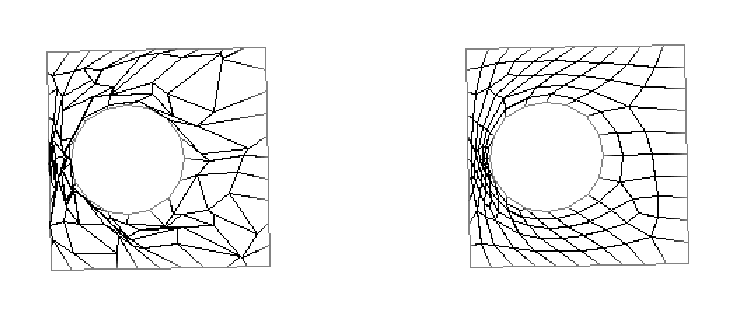
\includegraphics{hole_in_square.ps}
    \caption{hole\_in\_square.vtk mesh. The original mesh is on the left, the mesh smoothed with
    Mesquite is shown on the right.}
    \label{fig:hole}
\end{center}
\end{figure*}


% alternative names
%\chapter{Telling Mesquite About Your Mesh}
\chapter{Mesquite Interactions with Your Mesh and Geometry}
\label{sec:meshes}

Mesquite is responsible for gathering information from the
application's mesh and geometry.  Because this must be as efficient as
possible, considerable attention has been given to the interface
between Mesquite and the application code.  Because Mesquite is
designed as a library to work on a broad assortment of mesh and
element types on complex geometrical domains, a general,
data-structure neutral API is needed.  In general, Mesquite requires
access to basic information about the mesh such as the number of
vertices and elements in the mesh, the vertex locations, and the
element connectivities.  To move the vertex locations, Mesquite needs
to set the vertex coordinate positions, and eventually, to perform
swapping operations Mesquite will need to add and delete various mesh
entities.  In addition, for smoothing meshes on complex surfaces,
access to operations on the underlying solid model such as normal
information and closest point information are required to ensure
vertices are constrained to the surface.

\section{Reading in a Mesh File} \label{sec:meshFiles}

The simplest way to start using mesquite is to read a mesh file in one of the format currently
supported by mesquite. Currently, mesquite has a class that implements its mesh access interface and
supports the VTK \cite{VTKbook, VTKuml} and EXODUS formats: \texttt{MeshImpl}, as shown in the tutorial (section
\ref{sec:tutMesh}). The functions \texttt{MeshImpl::read\_vtk()}
and \texttt{MeshImpl::read\_exodus()} can be used as template to read instead your own mesh format. This is not
recommended, since ultimately you want to run mesquite dynamically to interact with your mesh
database and implementing the Mesquite Mesh Interface (section \ref{sec:msq_mesh}) should require the same amount of work. 

If you plan to link in with the EXODUS proprietary library, you will need to define the following
compile option in Mesquite's Makefile.customize: 

  [{\bf EXODUS\_LIB\_DIR}] is an optional variable that holds the location of the Exodus II library. 
({\it E.g.,} EXODUS\_LIB\_DIR = \$\{MSQ\_BASE\_DIR\}/external/exodus/lib).

\section{Implementing the Mesquite Mesh Interface} \label{sec:msq_mesh}

%Most users will want to skip this section and avoid the associated work. There are several manners
%to give the mesh data to Mesquite, and implementing the Mesquite mesh interface is the one that
%requires the most coding work. 
%
%Let's review the alternative in the first place. For very simple meshes, Mesquite has an integrated
%mesh database that can read in mesh files in specific format, such as VTK (see section \ref{sec:meshFiles}). 
%On the other hand, Mesquite is compatible with the TSTT mesh interface: this means that if you are
%running a code that has implemented the TSTT mesh interface, you can link Mesquite with your code
%and perform all mesh improvements through the TSTT mesh interface (see section \ref{sec:TSTT}).
%Implementing the TSTT mesh interface also has the advantage that your code will be compatible with
%the TSTT mesh interface standard: this is a very good investment. 
%
%If you want to implement the specific Mesquite mesh interface, you probably have very specific
%reasons in mind ... and you know what you are doing. In this section, we will give you the
%documentation for the abstract classes. This will allow you to implement the interface. 

\subsection{Mesh Interface Concepts}

To expose this information, Mesquite defines a set of interfaces 
(C++ abstract base classes) that are specifically designed for mesh
quality improvement needs.  There are four such interfaces: \texttt{Mesh},
\texttt{VertexIterator}, \texttt{ElementIterator}, and \texttt{MeshDomain}.
\begin{itemize}
\item \texttt{Mesh}: The Mesh interface represents the set of mesh
entities that are to be operated on.  It is through this interface
that one retrieves information about the mesh and its entities.
Examples of functionality provided by this interface include:
retrieving the number of elements in the mesh, determining which
elements contain a particular vertex, and modifying vertex
coordinates.
\item \texttt{VertexIterator}: The VertexIterator provides access to each
vertex in a mesh.  A VertexIterator is obtained from a Mesh object,
and is used to iterate through the list of all vertices in the Mesh
from which it was obtained.
\item \texttt{ElementIterator}: The ElementIterator provides access to
each element in a mesh.  Other than the type of entity it exposes, it
is identical to the VertexIterator.
\item \texttt{MeshDomain}: The MeshDomain represents the set of geometric
domains to which the mesh may be constrained. Its implementation is \emph{not} systematically 
required. See section \ref{sec:geometry} for more details. 
%The MeshDomain
%interface enables an application to restrict the locations to which a
%vertex can be moved, such as constraining a vertex to a surface.
%Through the MeshDomain interface, Mesquite's algorithms can also
%obtain a domain's normal vector, which aides validity checking and 
%decision making during the quality improvement process.
\end{itemize}
These interfaces are data-structure neutral and use only primitive
data types; an application may implement the Mesquite interfaces
without changing its existing mesh data structures.  Instead of
representing mesh entities with complex data structures or with typed
pointers, entities are identified with opaque values called handles.
Each mesh entity has a unique handle value, but otherwise handles have
no intrinsic meaning to Mesquite.  

\subsection{Implementation Details}

The implementation details must be looked up in the doxygen documentation located in mesquite/doc/developer.

\subsection{Testing Your Implementation}

The implementation of the Mesquite mesh interface is considerably eased by using the unit testing
framework. From the mesquite/testSuite/unit directory, change the MeshInterfaceTest.cpp file to
instantiate your mesh interface implentation (i.e. replace occurences of \texttt{MeshImpl} with your
class). Run gmake and run the test:
\begin{verbatim} 
./msq_test MeshInterfaceTest
\end{verbatim} 
This should help you pinpoint the vast majority of implementation errors. 


\section{Linking Mesquite with Implementations of the TSTT Mesh Interface} 
\label{sec:TSTT}

Mesquite can instead use the mesh interfaces currently
being developed through the TSTT center.  This interface definition
effort focuses on providing access to information pertaining to low
level mesh objects such as vertices, edges, faces, and regions through
both array-based and iterator-based mechanisms.  It is designed to
support existing packages such as CUBIT, NWGrid, PAOMD, and Overture. 
The TSTT interface achieves language interoperability
through use of the SIDL/Babel tools from LLNL \cite{babel}.
Achieving consensus within a large group of participants is
paramount (see \cite{Cubit-website}, \cite{overture}, \cite{aomd-imr},
and \cite{NWGrid-website}).  
%This interface definition effort is
%evolving, and the Mesquite team is actively participating to ensure
%that our needs for mesh quality improvement are adequately and
%efficiently addressed.  
A TSTT-based implementation of the Mesquite
interfaces is available.  As such, any tool that exposes its
mesh through the TSTT interfaces can be used with Mesquite without
additional development.

Note that the Mesquite-specific interface described in section \ref{sec:msq_mesh} is fully compatible
with the current TSTT mesh and geometry interfaces, and in fact,
Mesquite's approach to data structure neutrality is directly derived
from the TSTT interfaces.  Although similar in spirit to the TSTT
interface, the Mesquite-specific interface is not as general, and 
therefore consist of fewer
functions and does not require additional tools such as Babel.

\section{The Geometry Engine}
\label{sec:geometry}

Certain smoothing procedures in Mesquite require some geometry information. The mean ratio quality
metric for example requires the normal of a 2D element in a surface mesh. Also, boundary
vertices can be snapped back to the surface they belong to during a smoothing procedure, instead of
simply fixing the boundary vertices (and therefore lowering the quality of the final mesh). A simple abstract
class, \texttt{MeshDomain}, must be inherited and implemented by the user in order to provide the
geometry information to Mesquite.  This class contains only two virtual abstract functions:
\texttt{MeshDomain::normal\_at} and \texttt{MeshDomain::snap\_to} for which the details are given in
the doxygen documentation (in the directory mesquite/doc/developer).

Note that MeshDomain does not systematically needs to be implemented. For example it is possible to
improve a 3D mesh with any metric by fixing the boundary vertices. If the surface mesh is of good
quality but the volume mesh is poor, Mesquite can generates a high quality mesh without accessing
any geometry information. 


\subsection{The Simplified Geometry Engine}

We provide implementations of the MeshDomain class for basic geometries, such as a plan
(\texttt{PlanarDomain}) and a sphere (\texttt{SphericalDomain}). Those classes allows the user to use
Mesquite straight away without any implementation. They are introduced in the tutorial section
\ref{sec:tutMesh} and are described in details in the doxygen documentation.

\section{Visualizing the Mesh}

\begin{verbatim}
advices. pointer to VTK doc. 
pointer to VTK -> Exodus II converter
\end{verbatim}


\chapter{The Mesquite Application Programming Interface (API)} \label{sec:API}

Section \ref{sec:classesRelations} gives the details of the Mesquite paradigm. That section does not
delve into details and should be read before writing a driver code in order to master the basic
concepts. 

Section \ref{sec:detailedAPI} delves into the details of the various concrete classes available in
Mesquite. The syntaxic details of the API are given in the user doxygen doc available by running
'doxygen Mesquite-user.dox' in the directory mesquite/doc/user/doxygen. 

\section{Relations between the Mesquite API Classes} \label{sec:classesRelations}

The Mesquite architecture, shown in Figure \ref{fig:uml}, closely
follows the abstractions of the optimization problem defined in \ref{sec:concepts}.
In particular, the core abstract classes needed to
define a mesh quality improvement algorithm are {\tt QualityMetric},
{\tt ObjectiveFunction} (which takes a {\tt QualityMetric} as
input), and {\tt QualityImprover} (which takes an {\tt ObjectiveFunction}
as input).

In addition, a number of other classes have been created to support
the needs of mesh quality improvement algorithms:
\begin{itemize}
\item {\tt QualityAssessor}: to provide an evaluation of mesh
quality using standard statistical procedures,
\item {\tt TerminationCriterion}: to customize the stopping criteria
used with a mesh quality improvement algorithm,
\item {\tt InstructionQueue}: to compose quality improvers and
quality assessors together to form efficient mesh quality improvement
and evaluation methods, and
%\item {\tt MeshSet} and {\tt PatchData}: to provide the mechanisms
%for managing the application mesh and geometry information and the
%mesh sub-domains used in optimization procedures.
\end{itemize}

\subsection{UML Diagram}

\begin{figure*}[htbp]
\begin{center}
    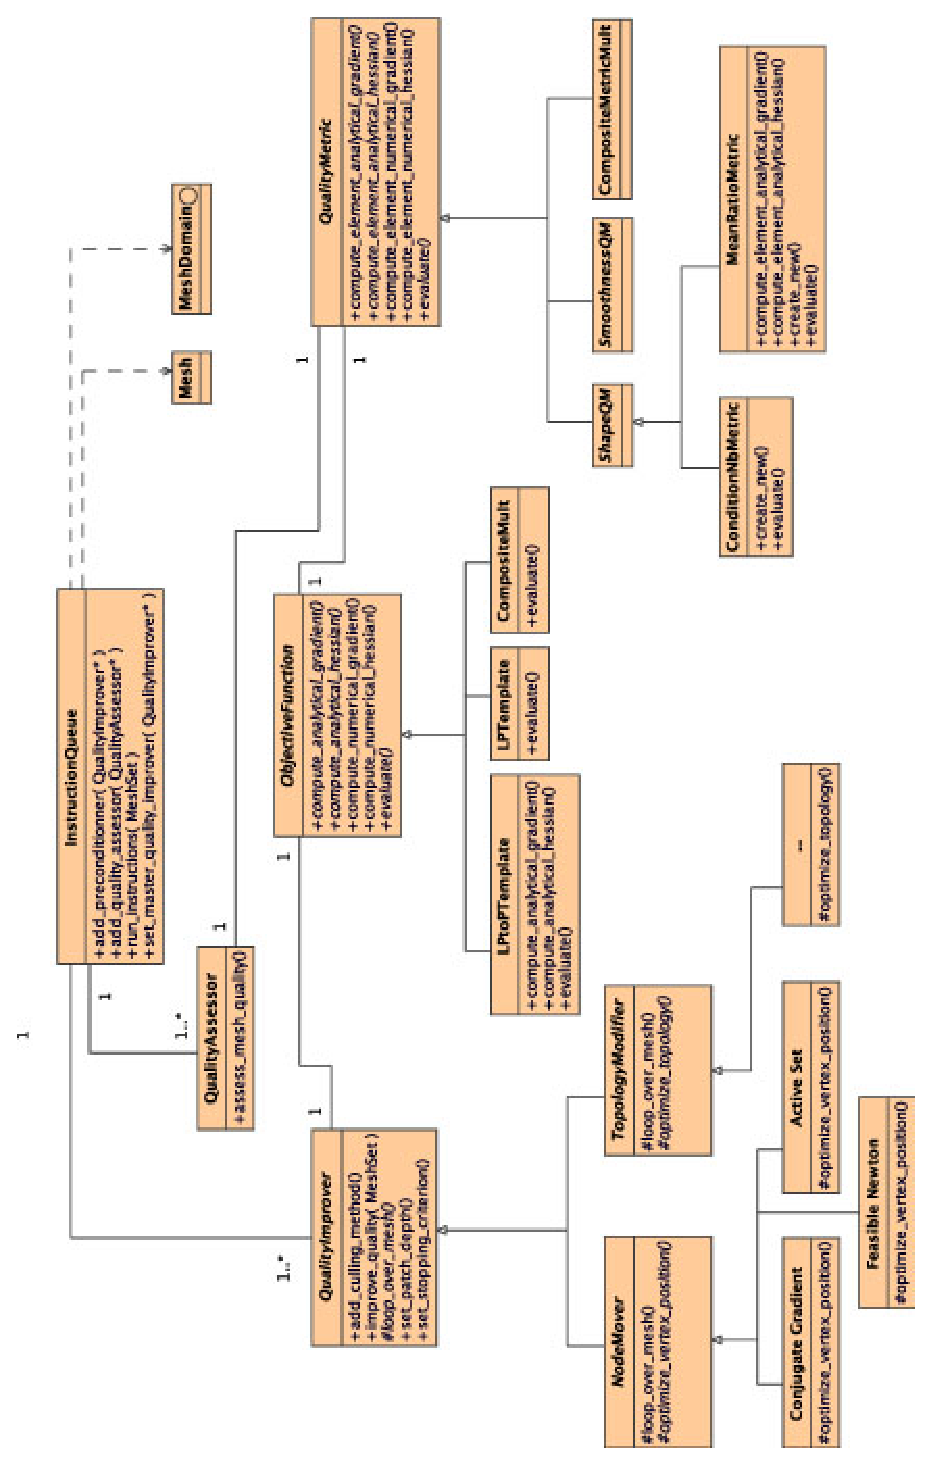
\includegraphics{MesquiteUI.eps}
    \caption{Mesquite user interface UML class diagram.  Abstract
             classes and virtual functions are in italic. Vertical
             links with a triangle indicate inheritance. Plain links
             indicate association. Protected functions are prefixed
             with '\#', public ones with '+' .}
    \label{fig:uml}
\end{center}
\end{figure*}

The UML diagram in figure \ref{fig:uml} presents the layout of the Mesquite classes. It should be
looked over once now, and then examined in more details when each class is described in the
following subsections.


\subsection{The Quality Metric -- Objective Function -- Quality Improver Trio} 
\label{sec:trio}

In the following sections, we will use the notations introduced in section \ref{sec:concepts}. 

Improving a mesh with Mesquite consists mainly in selecting three components: the quality metric,
the objective function template, ans the quality improver (i.e. the optimization algorithm). 

The quality metric $q$ describes what the user considers to be a good mesh element as a function of
its vertices coodinates, and possibly other factors such as its proximity to a boundary or an
equivalent element in a reference mesh. The various quality metrics available are described in
section \ref{sec:QualityMetric} and how to implement a new quality metric is described in section
\ref{sec:QualityMetricImpl}.

Now that the element quality has been defined, a template objective function $f$ (section
\ref{sec:ObjectiveFunction}) must be chosen to formulate the mesh we aim for. Do we want to improve
the worst elements, or to make the mesh as good as possible in average ? The combination of the
quality metric and the template objective function give us the mesh quality objective function $F=f
\circ q$.

This mesh quality objective function can now be minimized chosing an optimization algorithm
(\texttt{QualityImprover}), 
a crucial component of the Mesquite framework.  The two main types of improvement schemes
designed into Mesquite are {\tt VertexMover} (see section \ref{sec:VertexMover}) and {\tt
TopologyModifier} (\ref{sec:TopologyModifier}) for vertex relocation or topology modification,
respectively.  These methods take as input a mesh quality objective function ($F=f \circ q$).
The concrete \texttt{QualityImprover} always acts on an
\texttt{ObjectiveFunction} pointer to retrieve the function value and
gradient $\nabla F$, and sometimes the Hessian ${\cal H} F$, for a certain mesh and concrete \texttt{ObjectiveFunction} /
\texttt{QualityMetric} combination.  Dynamic polymorphism ensures at
runtime that the correct evaluations are performed.


\subsection{Termination Criterion}
\label{termination_section}

Mesquite's \texttt{TerminationCriterion} class contains functionality
to customize the termination of the mesh quality improvement process. 
Mesquite wrappers (section \ref{sec:wrappers}) already have an embedded default termination
criterion. The termination criterion provides an automatic mechanism to stop an optimization
procedure. --- familiar examples  comes to mind such as the objective function gradient norm close
to zero in a non-linear programming problem. Many other criterions are available in Mesquite (see
section \ref{sec:TerminationCriterion}). When using the detailed API, termination criterions have to
be set in order for the quality improver to terminate. 
 

\subsection{Quality Assessors}

Mesquite's \texttt{QualityAssessor} class encapsulates functionality to
evaluate quality metric values for a given mesh, to accumulate
statistical information about those values, and to report that data to
the user.  In particular, a \texttt{QualityAssessor} object takes a
{\tt QualityMetric} class as input to evaluate a given mesh and then
reports information like the maximum, average, and standard deviation
of those values.

% \subsection{Culling Capabilities} \label{sec:culling}
% Mesquite includes methods called {\it culling} schemes
% which are intended to decrease the time it takes for the
% quality improvers to reach an adequate mesh.  These schemes
% the mporarily fix the positions of certain vertices which
%satisfy a given culling criteria.  These fixed vertices
%are said to be {\it culled} from the optimization procedure.
%This reduces the number of variables in the optimization
%problem, and therefore this modified problem can often
%be solved in significantly less time than the original problem.  
% LAF - there are no details here - it's not worth including as is

%\subsection{Mesh Data Classes} \label{sec:MeshData}
%There are two mesh data classes in Mesquite, \texttt{MeshSet} and
%\texttt{PatchData}, which have been designed to meet two different
%needs.  The {\tt MeshSet} class is a container that holds pointers, or
%handles, to the meshes provided by the application.  It also provides
%the mechanisms necessary to obtain the mesh information from the
%application through a well-defined, flexible API (see Section
%\ref{sec:meshset}).  To minimize the memory footprint of the Mesquite
%library, only detailed information for the optimization procedure
%subdomains is stored at any given time in the {\tt PatchData} class.
%One or more {\tt PatchData} objects can be originated from the {\tt
%MeshSet} object, and {\tt PatchData} obtains detailed mesh
%information, such as vertex coordinates and element connectivity,
%through the MeshSet accessor functionality.  The \texttt{PatchData}
%class makes Mesquite scalable in that prohibitive memory costs
%associated with making a copy of a large application mesh can be
%avoided by dividing the mesh into patches on which to perform the
%optimization sequentially.
%\subsubsection{MeshSet Interactions with Application Meshes}
%\label{sec:meshset}
%\subsubsection{PatchData Interactions with QualityImprovers}
%Quality improvers are written to relocate nodes or modify topology
%within a \texttt{PatchData}, without any need to know whether the
%\texttt{PatchData} corresponds to the whole mesh or a subset of
%it. The \texttt{PatchData} information is generated by the
%\texttt{MeshSet} class with the \texttt{get\_next\_patch} function ---
%the equivalent of an iterator over a series of patches covering the
%mesh.  The user can set Mesquite to use different types of
%\texttt{PatchData}, ranging from a patch of elements containing one
%particular vertex to a patch of vertices connected to a central vertex
%through edges or a unique patch that covers the whole MeshSet
%(recall that this could be the union of several meshes added by the
%application to \texttt{MeshSet}).

%\texttt{PatchData} and its associated classes
%(e.g. \texttt{PatchDataVerticesMemento}) provides much functionality
%to the optimization algorithms.  Memento patterns can remember the
%state of a \texttt{PatchData} geometry or topology at a given
%iteration and restore the \texttt{PatchData} to that state
%later. Simple functions can move the \texttt{PatchData} $n$ vertices
%in a direction $d \in \Bbb{R}^{3n}$ while constraining the boundary
%vertices to their geometrical surface.

\subsection{The Instruction Queue} \label{sec:IQ}

The \texttt{InstructionQueue} class allows a sequence of operations
such as quality assessment and quality improvement to be performed on
a \texttt{MeshSet} object. The \texttt{InstructionQueue} 
provides a convenient framework to shield the user
from the algorithm syntax and to ensure a consistent use of the
Mesquite capabilities.  One or more quality improvers can be
associated with an {\tt InstructionQueue}, but one must be designated
as the {\it master} quality improver that determines the ultimate 
improvement goal.  All progress made by Mesquite will be
measured against the quality metrics set in the master quality
improver.  To improve the effectiveness and efficiency of the mesh
quality improvement process, several quality improvers can be used as
'pre-conditioners' for the master quality improver.  For example, a
user may precede an optimization-based master quality improver with a
mesh untangler and/or Laplacian smoothing.

Some predefined \texttt{InstructionQueue} objects, called \emph
{wrappers}, are available for high-level or novice users. Those
typically consist of a quality assessor, followed by a mesh
pre-conditioner such as an untangler, followed by a master quality
improver, and finally another quality assessor.  Once an
InstructionQueue has been defined, a single call to \texttt{run\_instructions} 
will perform all the contained operations.  We note
that once an \texttt{InstructionQueue} has been defined, it can be used
for several \texttt{MeshSet} objects.


\section{Simplified Application Programming Interface}
\label{sec:wrappers}
To improve meshes with a minimum of Mesquite function calls, we have 
provided a set of wrapper classes that encapsulate the 
most commonly used combination of quality metrics, improvement
algorithms and stopping criterion. Essentially, the wrappers are
inherited from the InstructionQueue, setting in their constructors
which algorithms to call. Using these wrappers, only
two lines of code are required to improve a \texttt{MeshSet}.

Wrappers do not provide access to low-level 
features such as setting a specific
termination criterion.  

\subsection{The Shape Improvement Wrapper}

The \texttt{ShapeImprovementWrapper} class 
first uses the mean ratio quality
metric (section \ref{sec:QualityMetric}) to assess and report the quality of the mesh elements. It then
untangles the mesh if necessary and improves the mesh with the
feasible Newton algorithm applied to the composition of the mean ratio
quality metric with the $\ell_2^2$ objective function (section \ref{sec:ObjectiveFunction}). Finally, the
mesh quality is assessed and reported again. 


\section{Detailed Application Programming Interface}
\label{sec:detailedAPI}

\subsection{Quality Metric} \label{sec:QualityMetric}

{\it 
What is a quality metric? Define full range, acceptable range, what is means 
if the metric uses a map, nodal-invariance, well-posed metrics, averaging 
methods, sample points. Give a list of the individual metrics we support. 
Provide a key to the tables.
}

\subsubsection{Concept}

In Mesquite, the \texttt{QualityMetric} class provides a measure of
the quality of individual mesh entities.  Quality metrics can evaluate
either element quality (for example, the mean ratio shape quality
metric) or vertex quality (for example, the sum of the adjacent edge
lengths squared can be used as a measure of vertex smoothness).  

In addition to the quality metric function value, the {\tt
QualityMetric} class also provides the gradient and Hessian
information needed for many optimization algorithms.  Numerical
approximations of the gradient and Hessian are automatically provided
by the \texttt{QualityMetric} base class.  Users can optionally
implement analytical expressions which are potentially more
computationally efficient.  For example, in the case of the mean ratio
quality metric implementation, the analytic calculation is
approximately twice as fast for the gradient and five times faster for the Hessian
as the numerical computation although this
improved efficiency often comes at a higher implementation cost.  The
cost of implementing the analytical gradients and Hessians can often
be alleviated, however, by the use of automatic differentiation tools
(for example, \cite{bischofadic}).

Mesquite also allows the user to scale metric values or combine
multiple metrics together to form a composite metric.  However, only
metrics which are evaluated on the same type of mesh entity can be
composed together.  That is, Mesquite does not allow element-based
metrics and vertex-based metrics to be added or multiplied together
because the result is not a meaningful measure of either element or
vertex quality.

\subsubsection{Currently Available Quality Metrics}  
Quality metrics within
Mesquite are grouped by the type of mesh properties that they measure.
Currently, there are four property groups: shape, smoothness, volume,
and untangle.  Composite metrics which allow the user to combine
multiple metrics or to scale metrics are given a separate group,
composite.  Future Mesquite development will include the
implementation of metrics falling under other group headings such as
orthogonality, shear, and alignment.  Table \ref{current-metrics}
lists the quality metrics currently available within Mesquite.  For
detailed definitions of the metrics, see \cite{Kn01}.  We note that
the implementation of the mean ratio metric has been extensively
optimized, and analytical gradients and Hessians are available for
that function.  Other metrics currently use numerical gradients and
Hessians.

The two composite metrics which are currently implemented
allow users to either multiply two metrics' values
together or raise a single metric's value to a given power.
The latter allows for negative powers and can therefore be used
to obtain the inverse of any Mesquite quality metric.  

\begin{table*}[htb]
\begin{center}
\begin{tabular}{|l|c|c|c|c|}
\hline
Metric & Group & Mesh Type & Feasibility Region &Entity Type\\
\hline
Area Smoothness &Smoothness & Any & No & Elements\\
Aspect Ratio & Shape &Tri/Tet & No & Elements\\
Composite Mult. & Composite &Any& Yes/No & Either\\
Composite Power & Composite &Any& Yes/No & Either\\
Cond. Num.& Shape & Any & Yes & Elements \\
Corner Jacobian & Volume & Any & No & Elements \\
Edge Length &Smoothness & Any & No & Vertices \\
Edge Length Range & Smoothness & Any &No & Vertices\\
Mean Ratio &Shape & Any & Yes &Elements\\
Untangle Beta &Untangle &Any&Yes&Elements\\
Vert. Cond. Num.& Shape & Any & Yes & Vertices\\
\hline
\end{tabular}
\label{current-metrics}
\caption{List of the current Mesquite quality metrics. The table also
indicates the metric group, the mesh types for which the metric is
valid, whether the metric is only valid within a feasible
region, and the type of entity for which the metric is defined (elements
or vertices).  Note that there may be a feasible region for composite
metrics depending on whether the underlying metrics require such a
constraint.}
\end{center}
\end{table*}


\begin{table}[h]
\begin{center}
\begin{tabular}{|l|c|c|c|c|c|}
\hline
Metric Name & Type & Dimension & Full Range & Ideal & Degenerate \\ \hline
Inverse Mean Ratio & Shape & 2D, 3D & $[0,1]$ & 1 & 0 \\ 
Mean Ratio &  &  &  &  &  \\ 
Condition Number &  &  &  &  &  \\ 
Untangle &  &  &  &  &  \\ 
Aspect Ratio Gamma &  &  &  &  &  \\ 
\hline
\end{tabular}
\caption{\label{QualityMetrics1} Mesquite Quality Metrics Summary, Part I}
\end{center}
\end{table}

\begin{table}[h]
\begin{center}
\begin{tabular}{|l|c|c|c|c|c|c|}
\hline
Metric Name & Map? & Averaging & Sample Pts & Elements & Gradient & Source \\ \hline
Inverse Mean Ratio & No & Harmonic & Vertices & TQTH & Analytic & \\ 
Mean Ratio &  &  &  &  &  \\ 
Condition Number &  &  &  &  &  \\ 
Untangle &  &  &  &  &  \\ 
Aspect Ratio Gamma &  &  &  &  &  \\ 
\hline
\end{tabular}
\caption{\label{QualityMetrics2} Mesquite Quality Metrics Summary, Part II}
\end{center}
\end{table}

\noindent {\bf Mean Ratio Metric} \newline
Give description, formulas. 

\subsubsection{Composite Metrics}

\subsection{Objective Function} \label{sec:ObjectiveFunction}

\subsubsection{Concept}
Remember the notations introduced in section \ref{sec:concepts}:
for each element of the mesh, let there be an associated quality metric, 
$q_n$.  Define the vector 
\begin{equation}
Q = [ q_1, q_2, \ldots, q_n ]
\end{equation}
where $N$ is the number of elements in the mesh. \footnote{For vertex-based metrics, an equivalent vector can be defined for a
quality metric associated with each free vertex $(1 \dots M)$ in the mesh. An example of vertex-based
metric is the longest edge connected to a vertex.}

While the \texttt{QualityMetric} class provides a way to evaluate the
properties of individual mesh entities, the \texttt{ObjectiveFunction}
class provides a way of combining those values into a single number
for the domain of the optimization problem.  This domain can either be
the entire mesh or a sub-mesh containing a subset of the free vertices.
For example, one available objective function template $f$ is the $\ell_{2}^2$
function which is the standard $\ell_{2}$ vector norm squared.  
Given an element-based quality metric $q$ and a mesh sub-domain $E$, the mesh 
quality objective function $F$ would be the composition of the template
objective function and the quality metric function 
\begin{equation}
F({\bf x}) = f \circ q({\bf x}) = \sum_{i \in E} (q_i({\bf x}))^2 \;\; .
\end{equation}

Given a \texttt{QualityMetric} $q$ and a mesh sub-domain $E$, the
\texttt{ObjectiveFunction} derived class computes the value of 
$F$ and, for $f$ and $q$ satisfying the appropriate smoothness
conditions, the mesh quality objective function's gradient and Hessian
with respect to the vertex positions.  As with {\tt QualityMetric},
Mesquite allows the gradient of $F$ to be calculated either
analytically or numerically. Computing the gradient of $F$
numerically is computationally expensive but requires only the quality
metric values.  If the gradient is calculated analytically, the
first derivative of the template objective function $f'$ and the
quality metric gradient $\nabla q$ are both required.\footnote{The 
quality metric gradients $\nabla q$ can be provided either numerically 
or analytically.}
To obtain the gradient $\nabla F$, the chain rule is applied
\begin{equation}
\nabla F({\bf x}) = \amalg_{i \in E} \left[ \nabla q_i({\bf x}) 
 (f' \circ q({\bf x}) ) \right] \;\; ,
\end{equation}
where $ f' \circ q({\bf x})$ is a scalar and $\amalg_{i \in E}$ denotes the
assembly over all the elements or vertices, for element-based or 
vertex-based quality metrics respectively.
Due to the significant advantages in computational
cost, analytical gradients have been implemented for all of the
continuously differentiable template objective functions in Mesquite.
Furthermore, an analytical Hessian calculation has been implemented
for the $\ell_p^p$ template objective function.  

\begin{table}[htb]
\begin{center}
\begin{tabular}{|c|c|c|}
\hline
Function & Gradient & Hessian\\
\hline
$\ell_P^P$     & Ana./Num.&Ana.\\
$\ell_P$       & Ana./Num.& Not Avail.\\
$\ell_{\infty}$& Not Avail.& Not Avail.\\
Comp. Add      & Ana./Num.& Not Avail.\\
Comp. Mult.    & Ana./Num.& Not Avail.\\
Scalar Add     & Ana./Num.& Not Avail.\\
Scalar Mult.   & Ana./Num.& Not Avail.\\
\hline
\end{tabular}
\label{current-objfunc}
\caption{List of the current objective functions available within
Mesquite.  With each function is a description of the types of
gradient and Hessian information available (Analytical and/or Numerical
or Not Available).}
\end{center}
\end{table}

\subsubsection{Available Objective Functions}

\noindent {\bf The $\ell_p$ Template} \newline
Given $1 \leq p < \infty$, let
\begin{equation}
\| Q \|_p = ( \sum_{n=1}^N \mid q_n \mid^p )^{1/p}
\end{equation}
be the $\ell_p$ template objective function. We recommend using the next template, \
$\ell_p^p$ since the $\ell_p$ template has no analytical gradient / Hessian implemented in Mesquite.\newline

\noindent {\bf The $\ell_p^p$ Template} \newline
Given $1 \leq p < \infty$, let 
\begin{equation}
\| Q \|_p = ( \sum_{n=1}^N \mid q_n \mid^p )
\end{equation}
be the 
$\ell_p^p$ template. The $\ell_p^p$ Template has its analytical gradient and Hessian implemented in
Mesquite. With $p=1$, this is the ``workhorse'' template objective function in Mesquite when the \emph{average}
quality of the mesh is to be improved. Increasing the value of $p$ will put more weight in improving
the quality of the worst elements. 
\newline

\noindent {\bf The $\ell_{\infty}$ Template} \newline
The $\ell_{\infty}$ template is
\begin{equation}
\| Q \|_{\infty} = \max_{n=1,\ldots,N} \mid q_n \mid
\end{equation}


\subsection{Composite Objective Functions}

Mesquite has four composite objective functions.  These are
\texttt{CompositeOFAdd}, \texttt{CompositeOFMultiply}, \texttt{CompositeOFScalarAdd}, and
\texttt{CompositeOFScalarMultiply}.  This combination allows users
to combine two objective functions by adding or multiplying
their respective values or to adjust a single objective function
by adding a scalar value or by multiplying by a scalar value.  
The user can adjust the objective function to modify the
optimization problem or to make the objective function value
more easily interpreted.  Scaling objective function values
is often useful when using a termination criterion based on the
objective function values. Unlike the quality metrics, 
two objective functions can be combined
even if the underlying quality metrics are defined on different entity
types.  That is, an objective function which operates on a vertex-based
quality metric can be added to an objective function which operates
on an element-based quality metric.  This structure allows the user
to have the maximum flexibility in defining an objective function with
which to measure the quality of a mesh.

\begin{verbatim} analytic gradients / Hessians ??? \end{verbatim} 

\subsection{Vertex Mover} \label{sec:VertexMover}

\subsubsection{Concept}
The are two quality improver base classes in the Mesquite architecture: \texttt{VertexMover} and
\texttt{TopologyModifier}. VertexMovers have the ability to relocate optimally the mesh vertices,
given a quality metric and a template objective function, without changing the mesh topology.
One important aspect of vertex movers is
the ability to seamlessly perform an optimization of a whole mesh or
to perform a sequence of optimizations on sub-patches of the mesh.
This behavior is chosen by the user at the \texttt{QualityImprover}
level with the \texttt{set\_patch\_type} function. 

\subsubsection{Available Vertex Movers}

\begin{table}[h]
\begin{center}
\begin{tabular}{|l|c|c|c|c|c|}
\hline
Solver Name & Description & Templates & L/G & Num/Anal & Fixed Vertices? \\ \hline
Steepest Descent & Classical & $\ell_p$ & Both & Both & Yes \\
Conjugate Gradient & & & & & \\
Feasible Newton & & & & & \\
Active Set & & Own & & & \\
Laplace & & None & & & \\
Randomize & & None & & & \\
\hline
\end{tabular}
\caption{\label{Solvers} Mesquite Solver Summary}
\end{center}
\end{table}

{\bf Conjugate Gradient Algorithm } \newline
\label{append_conjgrad}
This algorithm requires only
the objective function value $F$ and the objective function gradient $\nabla F$. 
In Mesquite this is usually done by applying the chain rule to the
analytical gradient of the objective function given the numerical or
analytical gradients of the element (or vertices) quality metrics 
(example given in section \ref{sec:ObjectiveFunction}). 

The conjugate gradient algorithm
has a linear convergence property for most problems. By using the
Polak-Ribi\`ere scheme to select a search direction which is a
combination of the gradient at the current iteration with the gradient
from one or more previous iteration, it avoids the zigzagging behavior
exhibited by the steepest descent algorithm when the equal cost
surfaces of the objective function are elongated (e.g. in narrow
valleys). In Mesquite this algorithm can be used with mesh patches of
any size; thus it is appropriate for optimizing all node positions 
simultaneously for any combination of $C^1$ objective functions and
quality metrics (see \cite{FeasNewt} for more details). 

On the performance front, Conjugate gradient is memory efficient but converges slowly.
On one hand, the conjuguate gradient algorithm is a lot slower than the Feasible Newton algorithm
when analytical gradient and hessians are available for the quality metrics. On the other hand, the
memory footprint of the conjugate gradient algorithm is a lot smaller than for the feasible Newton 
algorithm, since no Hessian has to be stored. A rough estimate would be a memory 
footprint 2 times smaller for a tetrahedral mesh, and 8 times smaller for an hexahedral mesh.  
\newline

{\bf Feasible Newton Algorithm } \newline
\label{append_feasnewt}
Newton's method minimizes a quadratic
approximation of a non-linear objective function. The algorithm requires
the objective function value, its gradient, \emph{and} its Hessian information.
Again, in Mesquite this
is usually done by computing the analytical gradient and Hessian of
the objective function given the numerical or analytical gradients and
Hessians of the quality metrics.  Note that objective functions that
lead to non-sparse Hessians entail a prohibitive memory cost in
Mesquite.\footnote{$\ell_p$ for $p \geq 2$ is such a function. The
number of variables in the objective function is the number of degrees
of freedom of the mesh, which must be squared to obtain the number of
entries in a dense Hessian.}  Newton's method is known to converge
super-linearly near a non-singular local minimum.   
Mesh-optimization problems that are performed within the neighborhood of
the minimum are a perfect application for Newton's method. In
Mesquite this algorithm can be used with mesh patches of any size,
making it appropriate to optimize all vertex positions simultaneously
for any $C^2$ objective function with a sparse Hessian.  In practice,
users will often observe an order of magnitude improvement\footnote{The larger the mesh, the
more dramatic the speed improvement between conjugate gradient (linearly convergent) and feasible
Newton (super-linearly convergent).} in
computation time when using the feasible Newton algorithm instead of
the conjugate gradient algorithm, making feasible Newton a worthwhile
choice when applicable (see \cite{FeasNewt} for more details). \newline

{\bf Active Set Method } \newline
\label{append_activeset}
The active set algorithm has been
developed for non-continuously differentiable objective functions such
as those computing the maximum value of a quality metric within a
patch of elements. This method is based on a non-smooth steepest
descent algorithm which efficiently computes a search direction and
step size based on the gradients of the values contained in the active
set.  Currently, this algorithm works on a patch of triangular or 
tetrahedral elements that 
contain a single free vertex.  Repeated
sweeps over the free vertices in the mesh leads to overall mesh
improvement (see \cite{fp:ijnme00} for more details).

\subsection{Topology Modifier} \label{sec:TopologyModifier}

Topology modifiers are the second type of quality improvers, They allow for optimal topology
modifications of the mesh , using swapping, flipping, etc ... 

Not available at this time. 

\subsection{Termination Criteria}

\subsubsection{Concept}
With the exception of wrappers (section \ref{sec:wrappers}), Mesquite algorithms need to be told
when to stop iterating within a given optimization procedure. 
As mentioned previously, many quality improvement algorithms can
perform mesh optimization on either the global mesh or on sub-meshes.
In the later case, the algorithm must be capable of determining when
to terminate two processes: 1) the optimization on the sub-mesh and 2)
the looping over the sub-meshes.  Mesquite's
\texttt{TerminationCriterion} class has been designed to handle either
of these cases.  Therefore, in general, quality improvers use two
\texttt{TerminationCriterion} objects: one, called the {\it inner
criterion}, to terminate the optimization of the sub-mesh and
another, called the {\it outer criterion}, to terminate the looping
over the sub-meshes.  Typically, quality improvers that support both
local and global optimizations always use two termination criterion. 
The outer criteria is set to terminate the optimization process after
one iteration in the global case.

Note that an interrupt handler (Ctrl-C) is also available, see section \ref{sec:Ctrl-C}. 

\subsubsection{Available Termination Criterions}
A wide range of cost, quality, 
and progress-centric termination
criterion types have been studied. These criteria have two basic types - 
absolute or relative - depending on whether or not the criterion is scale 
dependent.  Fourteen of these have been
implemented in \texttt{TerminationCriterion}.  Among the implemented
types are criteria which terminate optimization procedures due to
exceeding a set number of iterations, exceeding an allotted amount of
time, or reaching a mesh with a sufficiently small objective function
gradient.  

Any combination of the available criteria can be set on a given
\texttt{TerminationCriterion} object with the \texttt{add\_criterion\_type\_with\_double} and 
the \texttt{add\_criterion\_type\_with\_int} functions.  Compound criteria types consist
of statements joined by 'OR', for which 
the optimization process will be terminated when {\it any} of
the criteria have been satisfied.\footnote{Currently we have found little use
for compound criteria joined by 'AND', but this also could be implemented.}

The \texttt{TerminationCriterion} object is then set on the \texttt{QualityImprover} concrete class
with the \texttt{set\_inner\_termination\_criterion} and the \texttt{set\_outer\_termination\_criterion}
functions. Note that setting an inner or outer criterion on a \texttt{QualityImprover} overwrites
the previous inner or outer criterion.

The list of available termination criterions follows; those are the possible value of the
\texttt{TCType} enum. Make sure to consult the doxygen documentation
in mesquite/doc/user/doxygen for a list up to date with your Mesquite release. 
\begin{description}
\item[GRADIENT\_\-L2\_\-NORM\_\-ABSOLUTE] checks the gradient $\nabla f $ of objective function  $f
: I\!\!R^{3N} \rightarrow I\!\!R $ against a double $d$  and stops when $\sqrt{\sum_{i=1}^{3N}\nabla
f_i^2}<d$
\item[GRADIENT\_\-INF\_\-NORM\_\-ABSOLUTE]
checks the gradient $\nabla f $ of objective function  $f : I\!\!R^{3N} \rightarrow I\!\!R $ against
a double $d$  and stops when $ \max_{i=1}^{3N} \nabla f_i < d $ 
\item[GRADIENT\_\-L2\_\-NORM\_\-RELATIVE]terminates on the j\_\-th iteration when
$\sqrt{\sum_{i=1}^{3N}\nabla f_{i,j}^2}<d\sqrt{\sum_{i=1}^{3N}\nabla f_{i,0}^2}$ That is, terminates
when the norm of the gradient is small than some scaling factor times the norm of the original
gradient. 
\item[GRADIENT\_\-INF\_\-NORM\_\-RELATIVE]terminates on the j\_\-th iteration when $\max_{i=1 \cdots
3N}\nabla f_{i,j}<d \max_{i=1 \cdots 3N}\nabla f_{i,0}$ That is, terminates when the norm of the
gradient is small than some scaling factor times the norm of the original gradient. (Using the
infinity norm.) 
\item[KKT] Not yet implemented.
\item[QUALITY\_\-IMPROVEMENT\_\-ABSOLUTE] Terminates when the objective function value is smaller
than the given scalar value.
\item[QUALITY\_\-IMPROVEMENT\_\-RELATIVE] Terminates when the objective function value is smaller
than the given scalar value times the original objective function value. 
\item[NUMBER\_\-OF\_\-ITERATES] Terminates when the number of iterations exceeds a given integer.
\item[CPU\_\-TIME] Terminates when the algorithm exceeds an allotted time limit (given in seconds). 
\item[VERTEX\_\-MOVEMENT\_\-ABSOLUTE] Terminates when a the maximum distance moved by any vertex
during the previous iteration is below the given value. 
\item[VERTEX\_\-MOVEMENT\_\-RELATIVE] Terminates when a the maximum distance moved by any vertex
during the previous iteration is below the given value times the maximum distance moved by any
vertex over the entire course of the optimization. 
\item[SUCCESSIVE\_\-IMPROVEMENTS\_\-ABSOLUTE] Terminates when the decrease in the objective function
value since the previous iteration is below the given value.
\item[SUCCESSIVE\_\-IMPROVEMENTS\_\-RELATIVE] Terminates when the decrease in the objective function
value since the previous iteration is below the given value times the decrease in the objective
function value since the beginning of this optimization process. 
\item[BOUNDED\_\-VERTEX\_\-MOVEMENT] Terminates when any vertex leaves the bounding box, defined by the given value, d. That is, when
the absolute value of a single coordinate of vertex's position exceeds d. 
\end{description}


\subsection{Culling Algorithms}

\subsection{Quality Assessment}

\subsection{Instruction Queue}
Setting the master quality improver, setting up and using preconditioners,
using quality assessors, running the instruction queue.

Note that launching instructions through an \texttt{InstructionQueue} also allows mesquite to take
advantage of potential synergies. 


\section{Mesquite Specific Mechanisms}

\subsection{The Error Object -- MsqError}
\label{sec:MsqError}

\subsection{Hints for Performance Profiling}

\begin{verbatim}
Use the InstructionQueue. 
\end{verbatim}

\subsection{Interrupt Mechanism -- Ctrl-C} \label{sec:Ctrl-C}

Mesquite provides an interrupt handler in order to gracefully exit an ongoing optimization. When
the user hits \texttt{Ctrl-C}, Mesquite will catch the interrupt request, signal so, wait for the
current iteration to finish, update the user mesh with the improved mesh, and finish executing the
driver code.  

\chapter{Extending Mesquite}  \label{sec:extensions}

\section{Mesquite Programming Framework}

\subsection{Mesquite Repository} 

The CVS repository is currently located on the unix NFS at mcs.anl.gov, for example log on to
'shakey.mcs.anl.gov' and go to the directory '/home/mesquite/cvs'; the name of the CVS module is
'mesquite'.

Access to the mesquite repository requires an Argonne MCS account, which can be granted through Todd
Munson, among others: tmunson@mcs.anl.gov .
One way to use the cvs directory at argonne is through the ssh protocol, i.e. define the environment
variable 'CVS\_RSH' to be 'ssh' and for example, checking out a working copy would require the
following command, where :ext: will require CVS to consult the 'CVS\_RSH' variable: 
\begin{verbatim}
cvs -d :ext:username@shakey.mcs.anl.gov:/home/mesquite/cvs co mesquite
\end{verbatim}

\subsection{Mesquite Makefile} 

The mesquite makefile is \emph{not} a recursive makefile, i.e. a makefile that tells sub-directories
to execute their own makefile. Instead, it includes all variables from sub-directories into one main
makefile located in the main mesquite/ directory and called GNUmakefile.

Here we describe simple procedures needed for code development.

\subsubsection{Adding a header file within an existing directory}

Since adding a header file (.hpp) does not require to compile an extra objet file, no action is
needed in order for the makefile to use the header file. Just run 'gmake clean; gmake' in order for
the makefile to rerun its symbolinc links section or altenatively, create a symbolic link manually from
'mesquite/includeLinks' to the new header file.

\subsubsection{Adding a file within an existing directory}

When adding a '.cpp' file to an existing directory,  one needs to notify the makefile that a new
object file (.o) needs to be compiled. This is not done automatically in order to provide some
versatility.

Simply edit the 'MakefileVariables.inc' file within the directory where your new .cpp file has been added. The first
variable defines the current directory, let's call it CURRENTDIR. The second variable describes the
sources in the present directory (let's call it CONTROLSRC): that's the variable you need to add
your new file name to. For example, the MakefileVariables.inc file used to start with: 
\begin{verbatim}
CURRENTDIR = $(srcdir)/dir1

CURRENTSRC = $(CURRENTDIR)/file1.cpp \
            $(CURRENTDIR)/file2.cpp
\end{verbatim}
and it now starts with:
\begin{verbatim}
CURRENTDIR = $(srcdir)/dir1

CURRENTSRC = $(CURRENTDIR)/file1.cpp \
            $(CURRENTDIR)/file2.cpp \
            $(CURRENTDIR)/file3.cpp
\end{verbatim}
That's it, you can now run gmake from the 'mesquite'directory 
and it will pick up all dependencies and include your new file in
the mesquite library.

\subsubsection{Adding a directory within the source tree}

To add a new directory to the source tree, you need two files 
in the new directory: the 'MakefileVariables.inc' file and
 the 'MakefileTargets.inc' file. For example, copy those files from 
 the mesquite/src/Control directory and replace the string 'CONTROL' in 
those two files by a string unique to your new directory (for example 
'CONTROLSRC' becomes 'NEWDIRSRC'). Make sure not to miss any querry/replace.

You can now define the new directory location and the new source files 
names in the 'MakefileVariables.inc' file, as explained in the 
previous section.

Finally, you need to add the new directory to the MODULENAMES variable in the main makefile
mesquite/GNUmakefile, and you can run gmake. 

\subsubsection{Adding a new driver code}

To add a new driver code (e.g. mesquite/testSuite/test\_1/main.cpp), 
copy to a new directory under 'mesquite/testSuite/' the
'mesquite/testSuite/test\_1/Makefile.inc' file and change 
within that file the string TEST1 to a new unique string. 
Now, add the new directory to the TESTNAMES variable within 
'mesquite/GNUmakefile'. 

To compile the new driver, go to the main 'mesquite/' directory and type:
\begin{verbatim}
gmake mesquite/yournewdir/main
\end{verbatim}
where main will be the executable name (note that this name can be 
changed in the third variable in Makefile.inc).


\subsection{Unit Test Suite Makefile}

The unit test suite, located in 'mesquite/testSuite/unit/' has its 
own makefile. It is not as robust as the main mesquite makefile and can 
be improved (it does not pick up all dependencies properly).

To compile the unit test suite, go into 'mesquite/testSuite/unit/' 
and type 'gmake'. 

As you modify the test suite and mesquite in parallel, you might 
need to use 'gmake clean; gmake' to pick up some dependencies ... 
or you could improve the makefile. 


\subsection{Directory Structure}

The base directory of the Mesquite project contains several
sub-directories which are intended to help keep the project's
files organized.  Some of the sub-directories themselves are
also sub-divided.  Below are descriptions of the first level
of sub-directories ({\it i.e.,} the directories contained in the
base directory).
\begin{enumerate}
\item doc:  Contains a version of this document and a version of
the developer's documentation generated with doxygen (TODO: acknowledge
doxygen).
\item include:  Contains the Mesquite header file, ``Mesquite.hpp.''
\item includeLinks:  Contains soft links to the other header files
used within Mesquite.  
\item lib:  The location where the Mesquite library, ``libmesquite.a,'' is
stored.
\item meshFiles:  Contains example meshes that are used in some of
the test cases.
\item mswindow:  Contains the project file for compiling with Visual C++
(TODO: VC++ trademark statement???).
\item obj:  The directory where the object files are placed.
\item src:  Contains the Mesquite source code and header files (except for
Mesquite.hpp).
\item testSuite:  Contains example driver codes which use Mesquite.  These
test cases can only be ran when linked with the correct libraries (generally,
AOMD or MDB).
\end{enumerate}

\subsection{Code Testing Framework}

Another integral part of the Mesquite framework is the code testing
infrastructure.  Several testing methodologies have been included
within Mesquite. Unit testing is extensively used to facilitate
development and ensure low-level robustness. Functional testing is
used to ensure that user case scenarios run smoothly.

We use a broad definition for unit tests in Mesquite. Any test
performed on a class without need for the entire Mesquite framework is
considered a unit test. This encompasses simple assertions like
checking the result of the multiplication of a matrix $A \in
\Bbb{R}^{3 \times 3}$ by a vector $v \in \Bbb{R}^{3}$ to more complex
assertions such as checking that a concrete \texttt{QualityImprover}
correctly repositions a free vertex in a simple patch for a given
objective function and quality metric.

Mesquite uses a readily available testing framework called CppUnit
\cite{cppunit} --- essentially the well known jUnit testing framework
ported to C++.  Using the unit testing methodology allows the
developers to write far more robust code.

Applications using Mesquite may also find the testing framework useful
when verifying their additions to the code. In particular,
applications that prefer to implement Mesquite's mesh interface
instead of using the TSTT mesh interface will want to
check their implementation with the corresponding unit test collection
available in Mesquite. In addition, analytic gradient and Hessian
implementations can be checked against the numerical version provided
by the {\tt QualityMetric} base class using readily available unit
tests.

In addition to unit tests, the Mesquite test suite also includes
a range of functional tests.  While these tests also use the
CppUnit framework, they differ from unit tests in that 
functional tests require the entire Mesquite framework.
The functional tests are complete and often complex mesh
optimization problems.  These tests are intended to ensure that
the individual units of the Mesquite code work together correctly.
Performing these tests not only helps
validate the code but also allows developers to evaluate the
effects of code modifications in terms of Mesquite's accuracy
and efficiency on `real world' problems.

\section{Defining New Concrete Classes}

\begin{verbatim}
Explain that we only mention the truly polymorphic extensions. 
Extensions that require not only an additional class, 
but also other changes in the code (switches) are 
not discussed int he user manual for now. This is a 
reference manual issue. Give explicit examples of difficult things. 
\end{verbatim}

The Mesquite architecture uses as much dynamic polymorphism in the
form of inheritance and virtual functions as is possible without
degrading performance.  This allows developers to add new
functionality to Mesquite by inheriting from the appropriate abstract
class and implementing its interface (i.e. its abstract virtual
functions).  We note that the mesh entities, defined by class {\tt
MsqMeshEntity}, are the only exception in our architecture.  Mesh
entities, i.e. triangles, tetrahedrons, quadrangles and hexahedrons,
are implemented in a single class, without the use of dynamic
polymorphism, to eliminate the performance impact of runtime
resolution.

\subsection{Adding a New Quality Metric} \label{sec:QualityMetricImpl}

The primary functionality associated with the {\tt QualityMetric}
class is the \texttt{evaluate\_element} or\texttt{evaluate\_vertex}  function which returns a single quality value
for a given mesh entity.

To implement a new quality metric, a user must inherit from the base
\texttt{QualityMetric} class and implement the `evaluate' function.
\texttt{ QualityMetric} provides a wide range of
functionality that allows the quality metrics to be defined in a
flexible way and therefore gives the user the ability to modify the
metric in a variety of ways.  For example, the condition number
quality metric for a quadrilateral or hexahedral element is computed
by evaluating the condition number at a number of sample points in the
element.  Mesquite allows the user to select which set of sample
points are used in this calculation ({\it e.g.}, the element's
vertices) and how these values are combined to form a single metric
value ({\it e.g.}, linear averaging).  Mesquite is currently being
extended to allow certain quality metrics to be referenced to a
non-isotropic element.

\subsection{Adding a New Objective Function}

\subsection{Adding a New Vertex Mover Algorithm}

A new vertex mover algorithm is defined by inheriting from the
\texttt{VertexMover} abstract class. The \texttt{VertexMover} class 
is an intermediate abstract classe, inheriting from the
\texttt{QualityImprover} class (see Figure \ref{fig:uml}),  which
essential functionality is to implement the \texttt{loop\_over\_mesh}
virtual function that shields the optimization algorithm developer
from the need to distinguish between local or global patches.  The
\texttt{VertexMover} base class also checks the outer termination
criterion to stop iterating over mesh subsets (see section
\ref{termination_section}) and updates the application mesh after
optimizing a patch.

The
gathering of the mesh information into the patch is
carried out by the \texttt{MeshSet} and \texttt{PatchData} classes, so that the
optimization algorithm receives the appropriate patch to improve
simply by inheriting from \texttt{QualityImprover}.  If needed, one can 
override the \texttt{set\_patch\_type} function to accept only specific
patch types.

\subsection{Adding a New Topology Modifier Algorithm}

\section{LGPL License}
\begin{verbatim}
    MESQUITE -- The Mesh Quality Improvement Toolkit
 
    Copyright 2004 Sandia Corporation and Argonne National
    Laboratory.  Under the terms of Contract DE-AC04-94AL85000
    with Sandia Corporation, the U.S. Government retains certain
    rights in this software.
 
    This library is free software; you can redistribute it and/or
    modify it under the terms of the GNU Lesser General Public
    License as published by the Free Software Foundation; either
    version 2.1 of the License, or (at your option) any later version.
 
    This library is distributed in the hope that it will be useful,
    but WITHOUT ANY WARRANTY; without even the implied warranty of
    MERCHANTABILITY or FITNESS FOR A PARTICULAR PURPOSE.  See the GNU
    Lesser General Public License for more details.
 
    You should have received a copy of the GNU Lesser General Public License
    (lgpl.txt) along with this library; if not, write to the Free Software
    Foundation, Inc., 59 Temple Place, Suite 330, Boston, MA  02111-1307  USA
  
    diachin2@llnl.gov, djmelan@sandia.gov, mbrewer@sandia.gov,
    pknupp@sandia.gov, tleurent@mcs.anl.gov, tmunson@mcs.anl.gov
    
\end{verbatim}


\chapter{Troubleshooting}

\chapter{Caveats, Limitations, and Disclaimers}

Input meshes may suffer quality dis-improvement in some cases due to
failures of the numerical algorithm. Users are advised to keep a copy
of their original mesh in case of such a failure.

\chapter{User Support}

{\it Mailing lists, web site, examples, tutorials (pointer to slides?), 
instructions on downloading the software (open source, preparing 
derivative works), referencing Mesquite.}

\chapter{The Mesquite Team}

The core Mesquite team consists of five people from Sandia
National Laboratories (SNL) and Argonne National Laboratory (ANL): \newline

Michael Brewer (SNL), \newline

Lori Freitag-Diachin (Co-PI, LLNL), \newline

Patrick Knupp (Co-PI, SNL),\newline

Thomas Leurent (ANL), and \newline

Darryl Melander (SNL).  \newline

\noindent In addition,
significant contributions to the software have been made by
Todd Munson (ANL) who developed the Feasible Newton Solver.

\chapter{The Mesquite Development Plan}

{\it Timeline for proposed additions to the software.}



\chapter{Appendices}

\section{Appendix A: Mesh Interface}
\label{append_mesh}

\newcommand{\entrylabel}[1]{
   {\parbox[b]{\labelwidth-4pt}{\makebox[0pt][l]{\textbf{#1}}\\}}}
\newenvironment{Desc}
{\begin{list}{}
  {
    \settowidth{\labelwidth}{40pt}
    \setlength{\leftmargin}{\labelwidth}
    \setlength{\parsep}{0pt}
    \setlength{\itemsep}{-4pt}
    \renewcommand{\makelabel}{\entrylabel}
  }
}
{\end{list}}

\subsection{Detailed Description}
A Mesquite::Mesh is a collection of mesh elements which are composed of mesh vertices. Intermediate objects are not accessible through this interface (where intermediate objects include things like the faces of a hex, or an element's edges).

\subsection{Member Function Documentation}
\index{Mesquite::Mesh@{Mesquite::Mesh}!element_get_attached_vertex_count@{element\_\-get\_\-attached\_\-vertex\_\-count}}
\index{element_get_attached_vertex_count@{element\_\-get\_\-attached\_\-vertex\_\-count}!Mesquite::Mesh@{Mesquite::Mesh}}
\subsubsection{\setlength{\rightskip}{0pt plus 5cm}virtual size\_\-t Mesquite::Mesh::element\_\-get\_\-attached\_\-vertex\_\-count (Element\-Handle {\em elem}, {\bf Msq\-Error} \& {\em err}) honest\hspace{0.3cm}{\tt  [pure virtual]}}\label{classMesquite_1_1Mesh_a17}


Gets the number of vertices in this element. This data can also be found by querying the element's topology and getting the number of vertices per element for that topology type. 

\index{element_get_attached_vertex_indices@{element\_\-get\_\-attached\_\-vertex\_\-indices}!Mesquite::Mesh@{Mesquite::Mesh}}
\subsubsection{\setlength{\rightskip}{0pt plus 5cm}virtual void Mesquite::Mesh::element\_\-get\_\-attached\_\-vertex\_\-indices (Element\-Handle {\em element}, size\_\-t $\ast$ {\em index\_\-array}, size\_\-t {\em array\_\-size}, {\bf Msq\-Error} \& {\em err})\hspace{0.3cm}{\tt  [pure virtual]}}\label{classMesquite_1_1Mesh_a19}


Identifies the vertices attached to this element by returning each vertex's global index. The vertex's global index indicates where that element can be found in the array returned by {\bf Mesh::get\_\-all\_\-vertices}. 

\index{element_iterator@{element\_\-iterator}!Mesquite::Mesh@{Mesquite::Mesh}}
\subsubsection{\setlength{\rightskip}{0pt plus 5cm}virtual Element\-Iterator$\ast$ Mesquite::Mesh::element\_\-iterator ({\bf Msq\-Error} \& {\em err})\hspace{0.3cm}{\tt  [pure virtual]}}\label{classMesquite_1_1Mesh_a6}


Returns a pointer to an iterator that iterates over the set of all top-level elements in this mesh. The calling code should delete the returned iterator when it is finished with it. If elements are added or removed from the {\bf Mesh} after obtaining an iterator, the behavior of that iterator is undefined. 

\index{elements_get_attached_vertices@{elements\_\-get\_\-attached\_\-vertices}!Mesquite::Mesh@{Mesquite::Mesh}}
\subsubsection{\setlength{\rightskip}{0pt plus 5cm}virtual void Mesquite::Mesh::elements\_\-get\_\-attached\_\-vertices (Element\-Handle $\ast$ {\em elem\_\-handles}, size\_\-t {\em num\_\-elems}, Vertex\-Handle $\ast$ {\em vert\_\-handles}, size\_\-t \& {\em sizeof\_\-vert\_\-handles}, size\_\-t $\ast$ {\em csr\_\-data}, size\_\-t \& {\em sizeof\_\-csr\_\-data}, size\_\-t $\ast$ {\em csr\_\-offsets}, {\bf Msq\-Error} \& {\em err})\hspace{0.3cm}{\tt  [pure virtual]}}\label{classMesquite_1_1Mesh_a18}


Returns the vertices that are part of the topological definition of each element in the \char`\"{}elem\_\-handles\char`\"{} array.

When this function is called, the following must be true:\begin{enumerate}
\item 
\char`\"{}elem\_\-handles\char`\"{} points at an array of \char`\"{}num\_\-elems\char`\"{} element handles.\item 
\char`\"{}vert\_\-handles\char`\"{} points at an array of size \char`\"{}sizeof\_\-vert\_\-handles\char`\"{}\item 
\char`\"{}csr\_\-data\char`\"{} points at an array of size \char`\"{}sizeof\_\-csr\_\-data\char`\"{}\item 
\char`\"{}csr\_\-offsets\char`\"{} points at an array of size \char`\"{}num\_\-elems+1\char`\"{}\end{enumerate}
When this function returns, adjacency information will be stored in csr format:\begin{enumerate}
\item 
\char`\"{}vert\_\-handles\char`\"{} stores handles to all vertices found in one or more of the elements. Each vertex appears only once in \char`\"{}vert\_\-handles\char`\"{}, even if it is in multiple elements.\item 
\char`\"{}sizeof\_\-vert\_\-handles\char`\"{} is set to the number of vertex handles placed into \char`\"{}vert\_\-handles\char`\"{}.\item 
\char`\"{}sizeof\_\-csr\_\-data\char`\"{} is set to the total number of vertex uses (for example, sizeof\_\-csr\_\-data = 6 in the case of 2 TRIANGLES, even if the two triangles share some vertices).\item 
\char`\"{}csr\_\-offsets\char`\"{} is filled such that csr\_\-offset[i] indicates the location of entity i's first adjacency in \char`\"{}csr\_\-data\char`\"{}. The number of vertices in element i is equal to csr\_\-offsets[i+1] - csr\_\-offsets[i]. For this reason, csr\_\-offsets[num\_\-elems] is set to the new value of \char`\"{}sizeof\_\-csr\_\-data\char`\"{}.\item 
\char`\"{}csr\_\-data\char`\"{} stores integer offsets which give the location of each adjacency in the \char`\"{}vert\_\-handles\char`\"{} array.\end{enumerate}
As an example of how to use this data, you can get the handle of the first vertex in element \#3 like this: 

\footnotesize\begin{verbatim}VertexHandle vh = vert_handles[ csr_data[ csr_offsets[3] ] ] 
\end{verbatim}\normalsize 


and the second vertex of element \#3 like this: 

\footnotesize\begin{verbatim}VertexHandle vh = vert_handles[ csr_data[ csr_offsets[3]+1 ] ] 
\end{verbatim}\normalsize 
 

\index{elements_get_topologies@{elements\_\-get\_\-topologies}!Mesquite::Mesh@{Mesquite::Mesh}}
\subsubsection{\setlength{\rightskip}{0pt plus 5cm}virtual void Mesquite::Mesh::elements\_\-get\_\-topologies (Element\-Handle $\ast$ {\em element\_\-handle\_\-array}, Entity\-Topology $\ast$ {\em element\_\-topologies}, size\_\-t {\em num\_\-elements}, {\bf Msq\-Error} \& {\em err})\hspace{0.3cm}{\tt  [pure virtual]}}\label{classMesquite_1_1Mesh_a21}


Returns the topologies of the given entities. The \char`\"{}entity\_\-topologies\char`\"{} array must be at least \char`\"{}num\_\-elements\char`\"{} in size. 

\index{get_all_elements@{get\_\-all\_\-elements}!Mesquite::Mesh@{Mesquite::Mesh}}
\subsubsection{\setlength{\rightskip}{0pt plus 5cm}virtual void Mesquite::Mesh::get\_\-all\_\-elements (Element\-Handle $\ast$ {\em elem\_\-array}, size\_\-t {\em array\_\-size}, {\bf Msq\-Error} \& {\em err})\hspace{0.3cm}{\tt  [pure virtual]}}\label{classMesquite_1_1Mesh_a4}


Fills array with handles to all elements in the mesh.

\begin{Desc}
\item[Parameters: ]\par
\begin{description}
\item[{\em 
array\_\-size}]Must be at least the number of elements. If less than the mesh number of elements, an error is set (and a partial copy is made). \end{description}
\end{Desc}


\index{get_all_vertices@{get\_\-all\_\-vertices}!Mesquite::Mesh@{Mesquite::Mesh}}
\subsubsection{\setlength{\rightskip}{0pt plus 5cm}virtual void Mesquite::Mesh::get\_\-all\_\-vertices (Vertex\-Handle $\ast$ {\em vert\_\-array}, size\_\-t {\em array\_\-size}, {\bf Msq\-Error} \& {\em err})\hspace{0.3cm}{\tt  [pure virtual]}}\label{classMesquite_1_1Mesh_a3}


Fills array with handles to all vertices in the mesh.

\begin{Desc}
\item[Parameters: ]\par
\begin{description}
\item[{\em 
array\_\-size}]Must be at least the number of vertices. If less than the mesh number of vertices, an error is set (and a partial copy is made). \end{description}
\end{Desc}


\index{release@{release}!Mesquite::Mesh@{Mesquite::Mesh}}
\subsubsection{\setlength{\rightskip}{0pt plus 5cm}virtual void Mesquite::Mesh::release ()\hspace{0.3cm}{\tt  [pure virtual]}}\label{classMesquite_1_1Mesh_a23}


Instead of deleting a {\bf Mesh} when you think you are done, call {\bf release()} {\rm (p.\,\pageref{classMesquite_1_1Mesh_a23})}. In simple cases, the implementation could just call the destructor. More sophisticated implementations may want to keep the {\bf Mesh} object to live longer than {\bf Mesquite} is using it. 

\index{release_entity_handles@{release\_\-entity\_\-handles}!Mesquite::Mesh@{Mesquite::Mesh}}
\subsubsection{\setlength{\rightskip}{0pt plus 5cm}virtual void Mesquite::Mesh::release\_\-entity\_\-handles ({\bf Entity\-Handle} $\ast$ {\em handle\_\-array}, size\_\-t {\em num\_\-handles}, {\bf Msq\-Error} \& {\em err})\hspace{0.3cm}{\tt  [pure virtual]}}\label{classMesquite_1_1Mesh_a22}


Tells the mesh that the client is finished with a given entity handle. 

\index{vertex_get_attached_element_count@{vertex\_\-get\_\-attached\_\-element\_\-count}!Mesquite::Mesh@{Mesquite::Mesh}}
\subsubsection{\setlength{\rightskip}{0pt plus 5cm}virtual size\_\-t Mesquite::Mesh::vertex\_\-get\_\-attached\_\-element\_\-count (Vertex\-Handle {\em vertex}, {\bf Msq\-Error} \& {\em err}) const\hspace{0.3cm}{\tt  [pure virtual]}}\label{classMesquite_1_1Mesh_a15}


Gets the number of elements attached to this vertex. Useful to determine how large the \char`\"{}elem\_\-array\char`\"{} parameter of the {\bf vertex\_\-get\_\-attached\_\-elements()} function must be. 

\index{vertex_get_byte@{vertex\_\-get\_\-byte}!Mesquite::Mesh@{Mesquite::Mesh}}
\subsubsection{\setlength{\rightskip}{0pt plus 5cm}virtual void Mesquite::Mesh::vertex\_\-get\_\-byte (Vertex\-Handle {\em vertex}, unsigned char $\ast$ {\em byte}, {\bf Msq\-Error} \& {\em err})\hspace{0.3cm}{\tt  [pure virtual]}}\label{classMesquite_1_1Mesh_a13}


Retrieve the byte value for the specified vertex or vertices. The byte value is 0 if it has not yet been set via one of the \_\-set\_\-byte() functions. 

\index{vertex_is_fixed@{vertex\_\-is\_\-fixed}!Mesquite::Mesh@{Mesquite::Mesh}}
\subsubsection{\setlength{\rightskip}{0pt plus 5cm}virtual bool Mesquite::Mesh::vertex\_\-is\_\-fixed (Vertex\-Handle {\em vertex}, {\bf Msq\-Error} \& {\em err})\hspace{0.3cm}{\tt  [pure virtual]}}\label{classMesquite_1_1Mesh_a7}

Returns true or false, indicating whether the vertex is allowed to be repositioned. True indicates that the vertex is fixed and cannot be moved. Note that this is a read-only property; this flag can't be modified by users of the Mesquite::Mesh interface. 

\index{vertex_is_on_boundary@{vertex\_\-is\_\-on\_\-boundary}!Mesquite::Mesh@{Mesquite::Mesh}}
\subsubsection{\setlength{\rightskip}{0pt plus 5cm}virtual bool Mesquite::Mesh::vertex\_\-is\_\-on\_\-boundary (Vertex\-Handle {\em vertex}, {\bf Msq\-Error} \& {\em err})\hspace{0.3cm}{\tt  [pure virtual]}}\label{classMesquite_1_1Mesh_a8}


Returns true or false, indicating whether the vertex is on the boundary. Boundary nodes may be treated as a special case by some algorithms or culling methods. Note that this is a read-only property; this flag can't be modified by users of the Mesquite::Mesh interface. 

\index{vertex_iterator@{vertex\_\-iterator}!Mesquite::Mesh@{Mesquite::Mesh}}
\subsubsection{\setlength{\rightskip}{0pt plus 5cm}virtual Vertex\-Iterator$\ast$ Mesquite::Mesh::vertex\_\-iterator ({\bf Msq\-Error} \& {\em err})\hspace{0.3cm}{\tt  [pure virtual]}}\label{classMesquite_1_1Mesh_a5}


Returns a pointer to an iterator that iterates over the set of all vertices in this mesh. The calling code should delete the returned iterator when it is finished with it. If vertices are added or removed from the {\bf Mesh} after obtaining an iterator, the behavior of that iterator is undefined. 

\index{vertex_set_byte@{vertex\_\-set\_\-byte}!Mesquite::Mesh@{Mesquite::Mesh}}
\subsubsection{\setlength{\rightskip}{0pt plus 5cm}virtual void Mesquite::Mesh::vertex\_\-set\_\-byte (Vertex\-Handle {\em vertex}, unsigned char {\em byte}, {\bf Msq\-Error} \& {\em err})\hspace{0.3cm}{\tt  [pure virtual]}}\label{classMesquite_1_1Mesh_a11}


Each vertex has a byte-sized flag that can be used to store flags. This byte's value is neither set nor used by the mesh implementation. It is intended to be used by {\bf Mesquite} algorithms. Until a vertex's byte has been explicitly set, its value is 0. 


\chapter{Acknowledgments}

Mesquite is supported under the DOE SciDAC Terascale Simulation 
Tools and Technology (TSTT) project \cite{tstt}.  

{\it Funding sources (DOE SciDAC Program, Chuck Romine), Related activities
(TSTT, Cubit, Opt-MS), helpful folks (RPI for AOMD, TSTT for MDB, LLNL
for Overture tests, etc.}


\bibliographystyle{plain}
\bibliography{mesquite}


\end{document}

